\documentclass[a4paper]{article}

% CJK support: prefer ctex, fallback to XeTeX native line breaking
\IfFileExists{ctex.sty}{
  \usepackage[fontset=fandol]{ctex}
}{
  \usepackage{fontspec}
  \XeTeXlinebreaklocale "zh"
  \XeTeXlinebreakskip = 0pt plus 1pt
  \IfFontExistsTF{Songti SC}{\setmainfont{Songti SC}}{%
    \IfFontExistsTF{Noto Serif CJK SC}{\setmainfont{Noto Serif CJK SC}}{}%
  }
  \IfFontExistsTF{Heiti SC}{\setsansfont{Heiti SC}}{%
    \IfFontExistsTF{Noto Sans CJK SC}{\setsansfont{Noto Sans CJK SC}}{}%
  }
}

% Basic packages
\usepackage{amsmath, amssymb}
\usepackage{graphicx}
\usepackage[margin=2.5cm]{geometry}
\emergencystretch=3em
\usepackage[most]{tcolorbox}
\usepackage{etoolbox}
\usepackage{listings}
\usepackage{hyperref}
\hypersetup{hidelinks,pdftitle={南京大学生成式软件工程第13讲：软件分析工具},pdfauthor={lecture-to-notes}}
\usepackage{booktabs}
\usepackage{array}
\usepackage{subcaption}
\usepackage{float}
\usepackage{tikz}
\IfFileExists{pgfplots.sty}{
    \usepackage{pgfplots}
    \pgfplotsset{compat=1.18}
}{}

% ===== Highlight boxes =====
\newtcolorbox{knowledgebox}[1]{
    enhanced, colback=black!2!white, colframe=black!65, colbacktitle=black!65,
    coltitle=white, fonttitle=\bfseries, title={#1}, attach boxed title to top left={yshift=-2mm, xshift=2mm},
    boxrule=1pt, sharp corners
}

\newtcolorbox{importantbox}[1]{
    enhanced, colback=red!3!white, colframe=red!45!black, colbacktitle=red!45!black,
    coltitle=white, fonttitle=\bfseries, title={#1}, sharp corners
}

\newtcolorbox{warningbox}[1]{
    enhanced, colback=red!5!white, colframe=red!75!black, colbacktitle=red!75!black,
    coltitle=white, fonttitle=\bfseries, title={#1}, sharp corners
}

\newtcolorbox{practicebox}[1]{
    enhanced, colback=green!3!white, colframe=green!45!black, colbacktitle=green!45!black,
    coltitle=white, fonttitle=\bfseries, title={#1}, sharp corners
}

% ===== Code listings =====
\lstset{
    basicstyle=\ttfamily\small,
    keywordstyle=\color{blue},
    stringstyle=\color{red!60!black},
    commentstyle=\color{green!50!black},
    breaklines=true,
    frame=single,
    numbers=left,
    numberstyle=\tiny\color{gray},
    captionpos=b,
    extendedchars=false
}

% ===== Figure provenance and unit macros =====
\newcommand{\vtag}{\protect\footnotemark}
\newcommand{\srcnote}[1]{\footnotetext{视频画面时间区间：#1。若为裁剪图，时间区间仍对应原视频画面。}}
\newcommand{\degC}{\ensuremath{^{\circ}\mathrm{C}}}
\newcommand{\um}{\ensuremath{\mu\mathrm{m}}}
\newcommand{\nm}{\ensuremath{\mathrm{nm}}}
\newcommand{\angstrom}{\ensuremath{\text{\AA}}}

% ===== Front-page metadata =====
\newcommand{\notetitle}{软件分析工具}
\newcommand{\notesubtitle}{南京大学生成式软件工程 · 第 13 讲}
\newcommand{\noteauthors}{中文课程讲义 · lecture-to-notes}
\newcommand{\notedate}{2026 年 11 月 17 日}
\newcommand{\videochannel}{蒋炎岩主讲 / 绿导师原谅你了上传}
\newcommand{\videopublishdate}{20261117}
\newcommand{\videoduration}{91 分 33 秒}
\newcommand{\videourl}{https://www.bilibili.com/video/BV1wysu6hEkz/}
\newcommand{\videocoverpath}{cover.jpg}

\begin{document}

% ===== Title page =====
\begin{titlepage}
\centering
{\Large 课程笔记\par}
\vspace{1.2cm}
{\huge\bfseries \notetitle\par}
\ifdefempty{\notesubtitle}{}{
\vspace{0.3cm}
{\large \notesubtitle\par}
}
\vspace{0.5cm}
{\large \noteauthors\par}
\vspace{1.0cm}

\ifdefempty{\videocoverpath}{
{\small 请在生成笔记时填入视频封面图的本地路径。\par}
}{
\includegraphics[width=0.82\textwidth,height=0.40\textheight,keepaspectratio]{\videocoverpath}\par
}

\vfill
\begin{tcolorbox}[width=0.9\textwidth, colback=black!2!white, colframe=black!60, sharp corners]
\textbf{视频作者/频道}：\videochannel\par
\textbf{发布日期}：\videopublishdate\par
\textbf{视频时长}：\videoduration\par
\textbf{视频链接}：\ifdefempty{\videourl}{待填写}{\url{\videourl}}\par
\end{tcolorbox}
\end{titlepage}

% ===== Executive Summary =====
\newpage
\section*{执行摘要与核心脉络}

本讲义对应南京大学 2026 年秋季学期《生成式软件工程》（Generative Software Engineering）第 13 讲《软件分析工具》，由蒋炎岩老师主讲。在前两讲系统建立了软件质量保障的测试理论（\texttt{Fault $\to$ Error $\to$ Failure}）与形式化验证体系（Hoare 逻辑、模型检查、证明助手与 Curry--Howard 同构）之后，本讲站在整个计算机科学史与 AI 时代的交汇点，回答一个更具统摄性的元问题：\textbf{人类和智能体究竟是如何“用软件来改进制造软件的方法”的？面对 Rice 定理揭示的不可判定性铁幕，经典软件分析工具做出了怎样的工程取舍？当大语言模型将软件视为人类意图与习惯的概率分布采样时，下一代软件分析工具又将如何跨越形式化执行与人类世界之间的鸿沟？}

全讲围绕九个环环相扣的核心模块展开：
\begin{enumerate}
    \item \textbf{用软件改进制造软件的方法——软件工程三支柱与“人类 RSI”}：从“软件是物理世界过程在信息世界的投影”出发，梳理跨越 \texttt{Intent--Spec--Impl Gap} 的三大支柱——经验（《人月神话》、架构哲学、CMU SEI CERT C 安全编码规范）、流程（瀑布模型、敏捷开发、CI/CD）与工具。提出软件工具史本质上是一部“人类递归式自我改进（Recursive Self-Improvement，RSI）”的历史（如 GCC 编译器自举与 Engelbart 1991 三级改进模型），并在 AI 时代演进为智能体把单次推理沉淀为可复用工具（如 LATM, ICLR 2024）的闭环。
    \item \textbf{传统软件分析的“机械”本质与把程序作为数学对象}：剖析前大模型时代软件分析工具的共同前提——人类必须先把意图转化为明确的语法或形式语义规则（如用 CodeQL 将代码仓库抽取为包含 AST/CFG/SSA 的 Datalog 关系数据库并编写查询）。重温计算机科学的根基：以命令式语言 IMP 的大步求值与小步状态转移操作语义为基础，拆解软件测试（Oracle 判据）与编译器基本块插桩（\texttt{counter++}）统计 100\% 覆盖率的底层机制。
    \item \textbf{程序分析、形式化验证与 Rice 定理的不可判定性铁幕}：对比在抽象状态空间上计算的程序分析（以区间分析 $x \in [0,9] \Rightarrow y \in [1,10]$ 排除断言失败为例）与生成证明义务的程序验证；引入 1953 年 Rice 定理（不存在对任意程序总能停机并正确判定非平凡语义性质的通用算法），通过一段仅 4 行却等价于费马大定理（Wiles, 1995）的 Python 枚举程序，阐明为何完备且健全的万能分析器在数学上不可能存在，以及为何真实人类编写的信息系统只是所有可能程序空间中的极小良构子集。
    \item \textbf{Let's Trade Off（一）——静态分析工具的取舍（类型系统、Linter 与抽象解释）}：系统构建静态分析工具的“保留抽象--遗忘细节--知识来源”取舍矩阵。以 JavaScript 弱类型隐式转换（\texttt{0 == "0"}、\texttt{0 == []} 但 \texttt{"0" != []}）的非传递乱象对比 Rust/C++ 强类型系统，剖析 C 语言狂野强制类型转换（如将 \texttt{0x1234} 直接转为函数指针调用）的工程风险，并总结 Linter 覆盖 80\% 低级缺陷的六大高 ROI 类别。
    \item \textbf{Let's Trade Off（二）——动态执行与形式化模型取舍及强化学习反馈飞轮}：梳理动态工具（Fuzzing+Sanitizers、单元测试、QuickCheck 基于性质的测试、差分测试与 $\sin(-x) = -\sin(x)$ 蜕变测试）与模型验证工具（模型检验、符号执行、seL4 定理证明）的取舍矩阵。提炼“绿色对勾（Pass）买到了什么、红色告警（Fail）留下了什么”的证据判读表，并阐明基础工程卫生（缩进一致、清理 \texttt{a.out} 与 \texttt{.DS\_Store}）的贝叶斯信心信号以及工具链对大模型强化学习短程反馈飞轮的决定性意义。
    \item \textbf{把程序作为概率分布的采样——软件自然性与承载两个世界的代码}：打破“软件只是机械形式对象”的思维定势，引入 Hindle 等人（ICSE 2012《On the Naturalness of Software》）的软件自然性理论与 $N$-gram 马尔可夫统计模型，提出程序同时是条件概率分布 $\mathit{program} \sim P(\cdot \mid \mathit{intent}, \mathit{context}, \mathit{conventions})$ 的采样样本。通过课堂经典的“芒果 TV 访问控制函数”正反对比案例（从匿名代码 \texttt{f(x)} 还原为 \texttt{can\_watch\_huang\_guo\_tv(visitor)}），直观展示标识符命名如何将冰冷的布尔运算重新接回人类世界。
    \item \textbf{非形式化验证（Informal Verification）与“Mechanism Is King”}：解答“既然大模型如此强大，为何人类仍需要确定性软件”（CPU 确定性执行相比大模型推理拥有约 $10^9$ 即九个数量级的能效比优势）。正式定义面向未来的\textbf{非形式化验证（Informal Verification）}——检验形式化执行轨迹翻译回人类世界后是否符合 \texttt{intent} 与 \texttt{spec}；并借用 Jim Gray 在 06年提出的存储层次名言，确立 AI 时代软件分析的黄金法则：\textbf{``Heuristics is dead, Policy is Heuristics, LLM is Policy, Mechanism is King.''}
    \item \textbf{从日志挖掘、图形调试器到“No Doc”哲学——构建有“人感”的软件视图}：精读 Xu 等人在 SOSP 2009（2009年）发表的控制台日志挖掘论文（结合源码 AST 恢复日志模板并用 PCA 检测偏离正常模式的异常轨迹，如游戏穿模跌落 $z \to -\infty$），探讨“每条语句打日志以恢复非形式化语义（Informal Semantics）”的构想；现场编译演示 Andreas Zeller 的成名作 GNU DDD 图形调试器（1996），并提出 AI 时代的 \textbf{“No Doc”哲学}——凡是能从代码自动导出的结构描述均由 Skill 按需生成而不入库，文档只保留代码无法体现的架构取舍理由（Why，而非 What）。
    \item \textbf{软件工程工具的未来——三圆交集、架构泥潭与从第一性原理重构软件}：复盘主讲教师在 2024年绘制的“语法正确、阅读自然、语义正确”三圆维恩图，剖析当前 Coding Agent“初始采样 $+$ 工具反馈修补”范式的隐患——若初始采样架构错误，局部试错补丁会导致耦合激增并陷入无法维护的架构泥潭。展望十年内的终极形态：为智能体赋予“重理解需求（Re-understanding Intent）”“重写规约（Rewriting Spec）”与“沙盒演练需求变更”的一阶原语。
\end{enumerate}

\newpage
\tableofcontents
\newpage

% =========================================================================
% SECTION 1
% =========================================================================
\section{用软件改进制造软件的方法：软件工程三支柱与“人类 RSI”}

\subsection{软件是物理世界过程在信息世界的投影：经验、流程与工具}

“软件究竟是什么？”在本讲开篇，主讲教师给出了一个极具穿透力的第一性原理定义：\textbf{软件是物理世界过程在信息世界的投影}（对应配图）。我们在现实世界中所见的一切业务活动——无论是高校里的学生选课与成绩管理、电商平台的下单支付，还是录播教室的音视频推流——投射到比特构成的信息空间后，都化作了软件系统的状态与状态转移。

\begin{figure}[H]
\centering
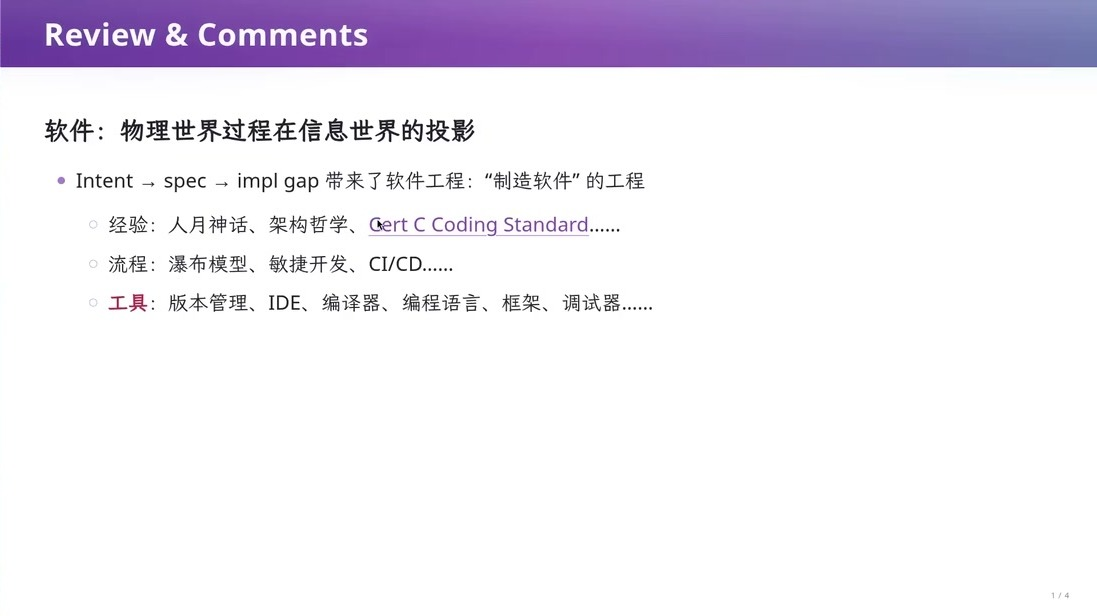
\includegraphics[width=0.88\textwidth]{figures/fig01_review_software_projection.jpg}
\caption{课程回顾：软件是物理世界过程在信息世界的投影，跨越 Intent--Spec--Impl Gap 依赖经验、流程与工具三大支柱\vtag}
\label{fig:fig01_review_software_projection}
\end{figure}
\srcnote{00:00:15--00:01:45}

然而，从人类脑海中模糊的愿望到最终在 CPU 上稳定运行的机器指令，中间横亘着两道巨大的鸿沟（对应配图）：
\begin{equation}
\underbrace{\text{Physical World}}_{\text{现实业务过程}}
\xrightarrow{\text{投影}}
\underbrace{\text{Intent（意图）}}_{\text{模糊自然语言}}
\xrightarrow{\text{Gap 1}}
\underbrace{\text{Spec（规格）}}_{\text{架构与契约}}
\xrightarrow{\text{Gap 2}}
\underbrace{\text{Impl（实现）}}_{\text{确定性状态机}}
\label{eq:projection_intent_spec_impl}
\end{equation}
在公式 \eqref{eq:projection_intent_spec_impl} 中，最顶层的 \textbf{Intent} 往往是高度模糊甚至自相矛盾的——就像那个经典的校园段子：“商学院同学拍脑袋想出了一个绝妙的商业模式，万事俱备，就差一个程序员了！”如果接手需求的新手程序员没有经过系统的工程训练，随便搭了一个脆弱的初始架构，那么随着需求迭代，最终写出来的 \textbf{Implementation} 就会偏离最初的 \textbf{Intent} 十万八千里。

\begin{figure}[H]
\centering

\includegraphics[width=0.72\textwidth]{figures/fig02_board_intent_spec_impl_triangle.jpg}
\caption{黑板板书：从顶层模糊意图（Intent）、中间规格说明（Spec）到底层代码实现（Implementation）的软件工程演化三角\vtag}
\label{fig:fig02_board_intent_spec_impl_triangle}
\end{figure}
\srcnote{00:01:00--00:01:40}

正是为了在无数次惨痛的软件失败中跨越 \texttt{Intent--Spec--Impl Gap}，人类在过去半个多世纪里沉淀出了软件工程的三大核心支柱：
\begin{enumerate}
    \item \textbf{经验（Experience）}：以 Fred Brooks 的《人月神话》（\textit{The Mythical Man-Month}）为代表，提醒我们软件复杂度随代码规模和团队人数呈非线性爆炸——构造一个 $10$ 万行软件的难度绝不是 $1$ 万行软件的 $10$ 倍，而可能是 $100$ 倍甚至更高。为了避免重蹈前人覆辙，工业界总结出了模块边界划分哲学以及极其详尽的安全编码规范。
    课堂上，主讲教师现场打开了卡内基梅隆大学软件工程研究所（CMU SEI）发布的 \textbf{SEI CERT C Coding Standard}（对应配图）：
    \begin{itemize}
        \item 在浮点数章节（\texttt{Floating Point, FLP}）中，规范逐条列出了诸如 \texttt{FLP30-C}（切勿使用浮点数作为循环计数器）、\texttt{FLP36-C}（大整数转浮点数时警惕精度丢失）等规则，并从严重度（Severity）、触发概率（Likelihood）与修复成本（Remediation Cost）三个维度给出了量化风险评估矩阵；
        \item 在字符串与字符章节中，主讲教师随机点开了 \textbf{\texttt{STR09-C: Don't assume numeric values for expressions with type plain character}}（对应配图）：由于 C 语言标准仅要求数字字符 `\texttt{'0'}`--`\texttt{'9'}` 具有连续递增的编码值，而并未规定普通 `\texttt{char}` 究竟是有符号（Signed）还是无符号（Unsigned），也没有强制所有平台必须使用 ASCII 编码（例如早期大型机使用 EBCDIC 编码，字母 `\texttt{'a'}`--`\texttt{'z'}` 编码甚至是不连续的！），因此除了相等比较（\texttt{==}, \texttt{!=}）和与 `\texttt{'0'}` 相减求数字值外，对普通字符做算术假设会导致严重的跨平台可移植性隐患。
    \end{itemize}
    \item \textbf{流程（Process）}：从早期强调严格阶段划分的瀑布模型（Waterfall Model），到拥抱快速迭代反馈的敏捷开发（Agile Development），再到现代工程强制要求的 Git \texttt{pre-commit} 门禁与 CI/CD 持续集成流水线。
    \item \textbf{工具（Tools）}：版本控制系统（Git）、集成开发环境（IDE）与智能体工作台（Agent Harness）、编译器、编程语言、框架与调试器——这是软件开发者最引以为傲的武器库。
\end{enumerate}

\begin{figure}[H]
\centering
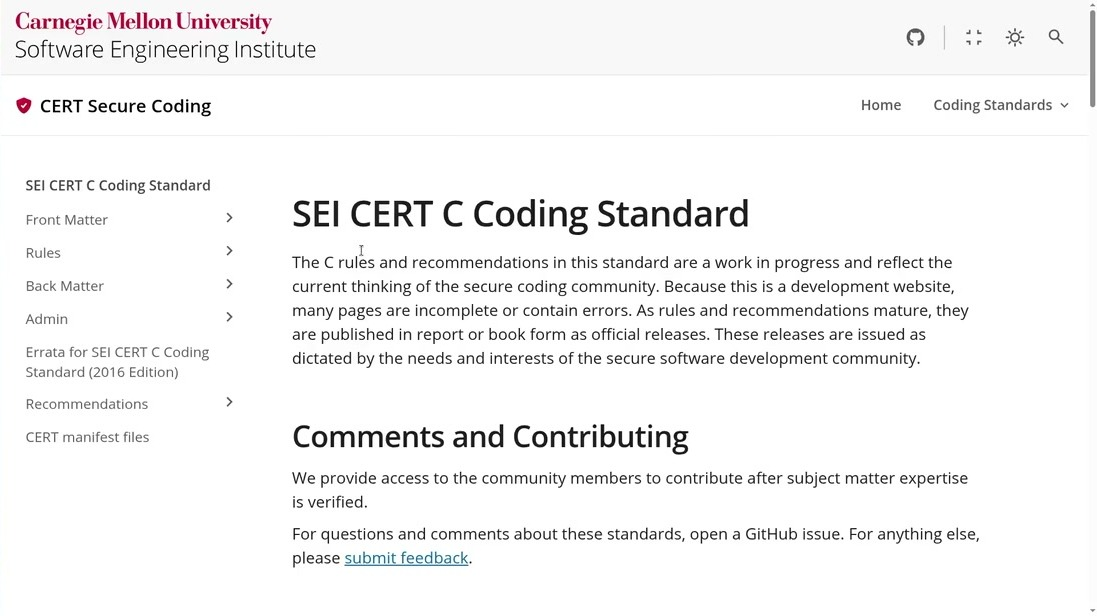
\includegraphics[width=0.82\textwidth]{figures/fig03_sei_cert_c_floating_point.jpg}
\caption{网页实机演示（一）：CMU SEI CERT C 编码规范中的浮点数（FLP）安全规则目录与风险评估等级表\vtag}
\label{fig:fig03_sei_cert_c_floating_point}
\end{figure}
\srcnote{00:02:00--00:02:20}

\begin{figure}[H]
\centering
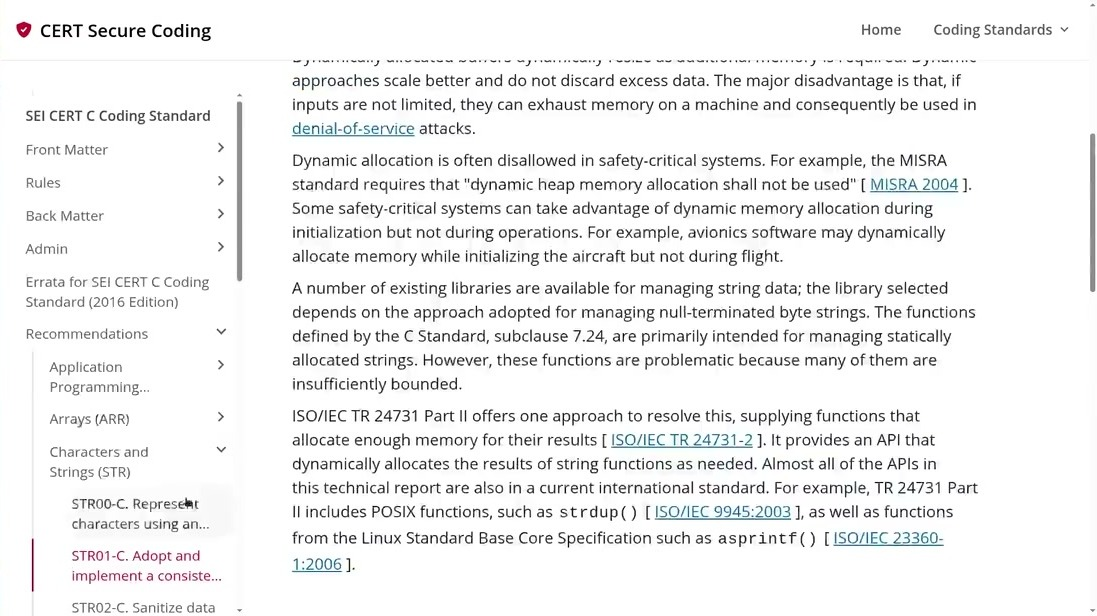
\includegraphics[width=0.82\textwidth]{figures/fig04_sei_cert_c_str09_char.jpg}
\caption{网页实机演示（二）：CERT C \texttt{STR09-C} 规则详解——为何不应假定普通字符（\texttt{plain char}）表达式的具体数值编码\vtag}
\label{fig:fig04_sei_cert_c_str09_char}
\end{figure}
\srcnote{00:02:25--00:02:50}

\subsection{工具与“人类 RSI”：从编译器自举、Engelbart 模型到 AI 自造工具}

为什么在所有工程学科中，唯独软件工程与工具的关系如此血脉相连？因为土木工程师造出的桥梁不能自动帮他画下一座桥的图纸，但\textbf{软件工程师造出的软件，其输入本身就可以是另一份软件（例如一个 \texttt{.git} 仓库、一个 \texttt{.c} 或 \texttt{.ts} 源文件）}！

回望软件工程的发展史，主讲教师将其精辟地概括为一部\textbf{“人类 RSI（Recursive Self-Improvement，递归式自我改进）”}的历史（对应配图）：

\begin{figure}[H]
\centering
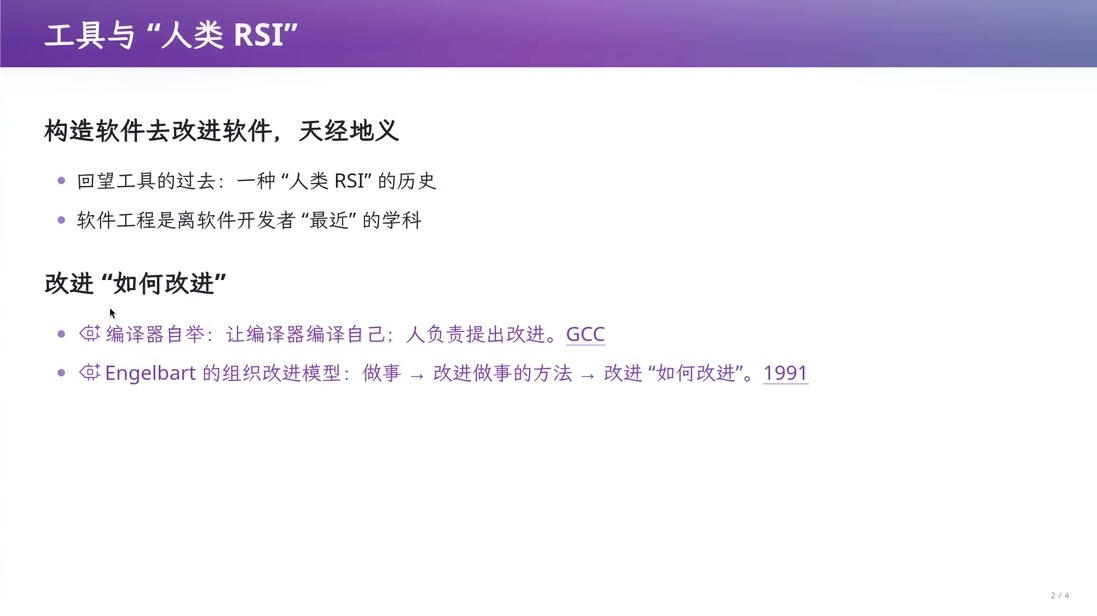
\includegraphics[width=0.88\textwidth]{figures/fig05_tools_and_human_rsi.jpg}
\caption{工具与“人类 RSI”：构造软件去改进软件天经地义——从 GCC 编译器自举到 Engelbart（1991）的三级组织改进模型\vtag}
\label{fig:fig05_tools_and_human_rsi}
\end{figure}
\srcnote{00:05:25--00:07:30}

\begin{itemize}
    \item \textbf{编译器自举（Compiler Bootstrapping）}：C 语言编译器（如 GCC）自己就是用 C/C++ 语言编写的。在最初没有 C 编译器时，先驱们先用汇编或机器码写一个能编译 C 语言极小子集的初级编译器 $C_0$；再用这个子集写出功能更完整的编译器源码并用 $C_0$ 编译得到 $C_1$；如此循环迭代，让编译器自己编译自己、自己优化自己。
    \item \textbf{Engelbart（1991）的三级改进模型（A / B / C Activity Model）}：鼠标与超文本的发明者 Douglas Engelbart 在 1991 年提出了著名的能力基础设施框架，将工程组织的活动划分为三个递进层级：
    \begin{equation}
    \underbrace{\text{A：做事（Core Work）}}_{\text{编写业务软件}}
    \longleftarrow
    \underbrace{\text{B：改进做事的方法}}_{\text{编译器、IDE、Linter}}
    \longleftarrow
    \underbrace{\text{C：改进“如何改进”}}_{\text{元工具与分析理论}}
    \label{eq:engelbart_abc_rsi}
    \end{equation}
    在传统软件工程中，“不安分的码农”每在日常开发（A 层）中踩过一次坑，就会把经验抽象成一个新的 IDE 插件、Linter 规则或单元测试可视化工具（B 层），从而提升自己的开发效率，进而腾出更多精力去制造更强大的工具。
\end{itemize}

而到了生成式 AI 时代，公式 \eqref{eq:engelbart_abc_rsi} 所示的 RSI 飞轮迎来了历史性的主角交接（对应配图）：当人们还在惊叹于大模型能否用 Three.js 一次性许愿生成类似 \textbf{3A} 大作的 3D 游戏时，更深层的质变在于——\textbf{AI Agent 已经开始具备把“本次任务的单次推理摸索”沉淀为“下次任务可直接调用的专用工具”的能力}（例如蔡天乐等人在 ICLR 2024 发表的 \textbf{LATM：Large Language Models as Tool Makers}）。

\begin{figure}[H]
\centering
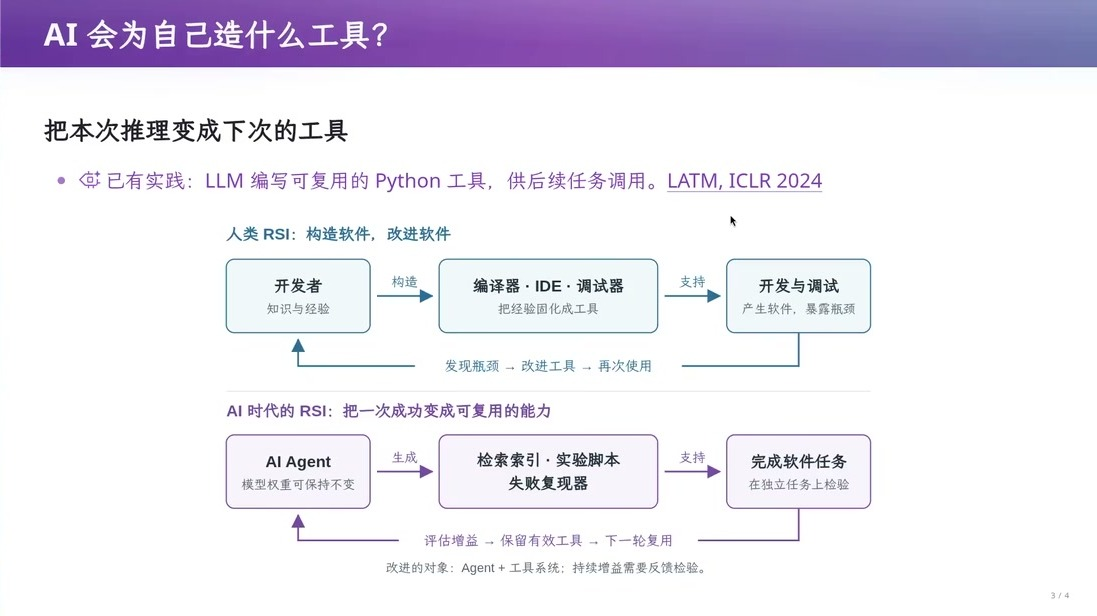
\includegraphics[width=0.88\textwidth]{figures/fig06_ai_tool_creation_latm.jpg}
\caption{AI 会为自己造什么工具：对比“人类 RSI（开发者 $\to$ 编译器/IDE/调试器 $\to$ 开发与调试）”与“AI 时代的 RSI（AI Agent $\to$ 检索索引/实验脚本/失败复现器 $\to$ 完成软件任务）”\vtag}
\label{fig:fig06_ai_tool_creation_latm}
\end{figure}
\srcnote{00:07:55--00:10:20}

\begin{importantbox}{人机两代 RSI 闭环的核心对比：从通用重型工具到任务定制微工具}
如对应配图所示，人类时代的 RSI 往往周期较长，沉淀出的是编译器、IDE、通用调试器等重型标准基础设施；而在 AI 时代的 RSI 闭环中，当 Agent 在排查一个棘手的系统 Bug 时，它可以当场编写一个专用的\textbf{检索索引脚本}、\textbf{最小失败复现器（Reproducer）}或\textbf{自动化实验探针}，并在任务完成后通过评估筛选将这些脚本持久化到项目的工具库（如 \texttt{scripts/} 或 \texttt{skills/}）中。这样一来，下一次 Agent 会话面对类似问题时就无需从零重复消耗 Token 摸索，真正实现了 $\text{Agent} + \text{工具系统}$ 的复利演进。
\end{importantbox}

% =========================================================================
% SECTION 2
% =========================================================================
\section{传统软件分析的“机械”本质与把程序作为数学对象}

\subsection{为什么说前 AI 时代的软件分析工具都是“机械”的？（以 CodeQL 为例）}

在探讨 AI 如何重塑软件分析之前，我们必须先看清传统软件分析工具的本质边界。在生成式 AI 出现之前，无论一个静态分析器、Linter 还是模型检查器背后的算法设计得多么精妙，它们在根本上都是\textbf{“机械”的（Mechanical）}（对应配图）：

\begin{figure}[H]
\centering
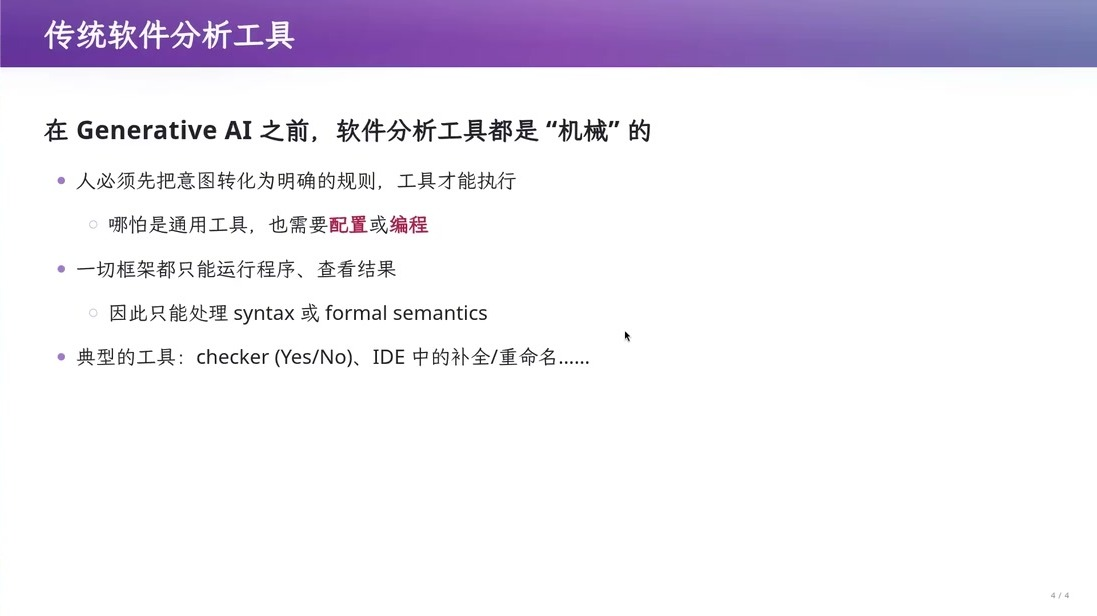
\includegraphics[width=0.88\textwidth]{figures/fig07_traditional_mechanical_tools.jpg}
\caption{传统软件分析工具的“机械”本质：人必须先把意图转化为明确的规则或配置，工具只能处理语法（Syntax）或形式语义（Formal Semantics）\vtag}
\label{fig:fig07_traditional_mechanical_tools}
\end{figure}
\srcnote{00:10:25--00:13:15}

为什么说是“机械”的？因为在传统计算机科学（数据结构、编译原理、数据库）的框架下，算法只能处理树（AST）、图（CFG/Call Graph）或关系表等严格结构化的符号对象，而完全无法直接理解人类脑海中的非结构化意图（\texttt{Intent}）或自然语言需求文档（\texttt{Spec}）。因此，\textbf{人类专家必须先充当“翻译官”，把模糊的工程经验转化为百分之百确定性的形式化规则（Rule-based Query），工具才能按部就班地执行检查。}

为了展示人类在“机械化规则分析”方向上达到的最高工程造诣，主讲教师在终端中现场调出了关于工业级声明式代码分析引擎 \textbf{CodeQL} 的技术笔记（对应配图）：

\begin{figure}[H]
\centering

\includegraphics[width=0.80\textwidth]{figures/fig08_codeql_llm_interface_notes.jpg}
\caption{终端技术笔记（一）：CodeQL 与生成式软件工程的结合——LLM 将人类怀疑翻译为声明式 QL 查询，在十万行代码库上执行精准污点分析\vtag}
\label{fig:fig08_codeql_llm_interface_notes}
\end{figure}
\srcnote{00:14:10--00:14:30}

\begin{figure}[H]
\centering
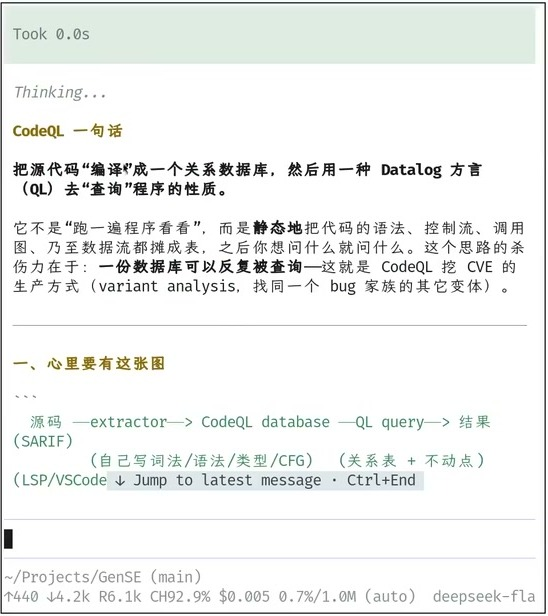
\includegraphics[width=0.80\textwidth]{figures/fig09_codeql_ast_cfg_schema_table.jpg}
\caption{终端技术笔记（二）：CodeQL 将源代码编译抽取为六类核心关系数据库表（\texttt{functions}、\texttt{exprs/stmts}、\texttt{variables}、\texttt{calls}、\texttt{basic\_blocks}、\texttt{ssa\_definitions}）\vtag}
\label{fig:fig09_codeql_ast_cfg_schema_table}
\end{figure}
\srcnote{00:14:35--00:15:20}

CodeQL 的核心思想非常优雅：\textbf{把一份静态源代码仓库（C/C++、Java、Python、TypeScript 等）编译抽取为一个只读的关系型数据库（Relational Database），然后让开发者用类似 SQL 的声明式逻辑查询语言（QL，底层基于 Datalog 不动点求值）去查询代码的语法与数据流性质！}如对应配图所示，CodeQL 提取出的数据库包含六张核心关系表：
\begin{table}[H]
\centering
\caption{CodeQL 静态分析数据库的核心关系模式（Schema）}
\label{tab:codeql_schema}
\begin{tabular}{p{3.5cm}p{9.8cm}}
\toprule
\textbf{关系表名（Relation）} & \textbf{存储的程序结构与语义事实（Extracted Facts）} \\
\midrule
\texttt{functions} & 每个函数的名称、参数签名、所属源文件及起止行号 \\
\texttt{exprs / stmts} & 每个表达式与语句节点，附带抽象语法树（AST）父子层级关系 \\
\texttt{variables / variable\_access} & 变量的声明点与每一处读写引用（如赋值目标或表达式读取） \\
\texttt{calls} & 函数/方法调用点 $\to$ 被调目标函数（已由前端完成函数重载消解与虚表初步绑定） \\
\texttt{basic\_blocks / cfg\_nodes} & 控制流图（CFG）的基本块划分及前驱/后继跳转边 \\
\texttt{ssa\_definitions} & 静态单赋值（SSA）形式的局部定义--使用链（Def-Use Chain） \\
\bottomrule
\end{tabular}
\end{table}

例如，如果我们想检查“同一个函数内调用 `\texttt{malloc}` 分配内存后是否遗漏了 `\texttt{free}`”，或者做跨函数的安全污点跟踪（Taint Tracking：定义外部不可信输入为 \texttt{source}、危险系统调用或 SQL 拼接为 \texttt{sink}），就可以编写如下声明式 QL 查询：
\begin{lstlisting}[language=SQL, caption={CodeQL 污点分析与规则查询概念结构}]
from DataFlow::Node source, DataFlow::Node sink
where MyTaintConfig::flow(source, sink)
select sink, "Untrusted data flows from $@ to dangerous sink.", source, source.toString()
\end{lstlisting}
\begin{practicebox}{工程实践：用 CodeQL 弥合大语言模型与十万行代码库之间的结构化鸿沟}
在大模型辅助审计大型项目时，直接让模型用 \texttt{grep} 搜索文本往往只能看到孤立碎片。更高效的范式是：让人类提供领域知识（什么是危险的 \texttt{source} 与 \texttt{sink}），让大模型将其翻译为几十行声明式 CodeQL 查询，再由 CodeQL 在 AST、CFG 与 SSA 关系表上一次性算出全部跨函数污点传播路径，从而把模型模糊的“怀疑”变成精确的静态检查器。
\end{practicebox}

在生成式软件工程时代，CodeQL 这类工具非但没有过时，反而成为了大模型绝佳的“结构化眼睛”：面对几十万行代码库，大模型如果直接靠 `\texttt{grep}` 搜索，极易漏掉跨文件别名传递或被海量无关文本淹没上下文；而如果由\textbf{人类或大模型负责提出领域假设并编写几行声明式 QL 查询（定义 \texttt{source}/\texttt{sink}/\texttt{sanitizer}），再交由 CodeQL 引擎执行底层的图可达性不动点计算}，就能把模糊的怀疑瞬间转化为百发百中的可执行检查器！

\subsection{把程序作为数学对象：IMP 语言的操作语义（Operational Semantics）}

无论工具如何演进，在进行“许愿编程”的同时，我们绝不能忘记计算机科学的数学根基：\textbf{程序的运行具有完全明确的规则，任何程序本质上都是一个数学对象（Mathematical Object）}（对应配图）。

\begin{figure}[H]
\centering
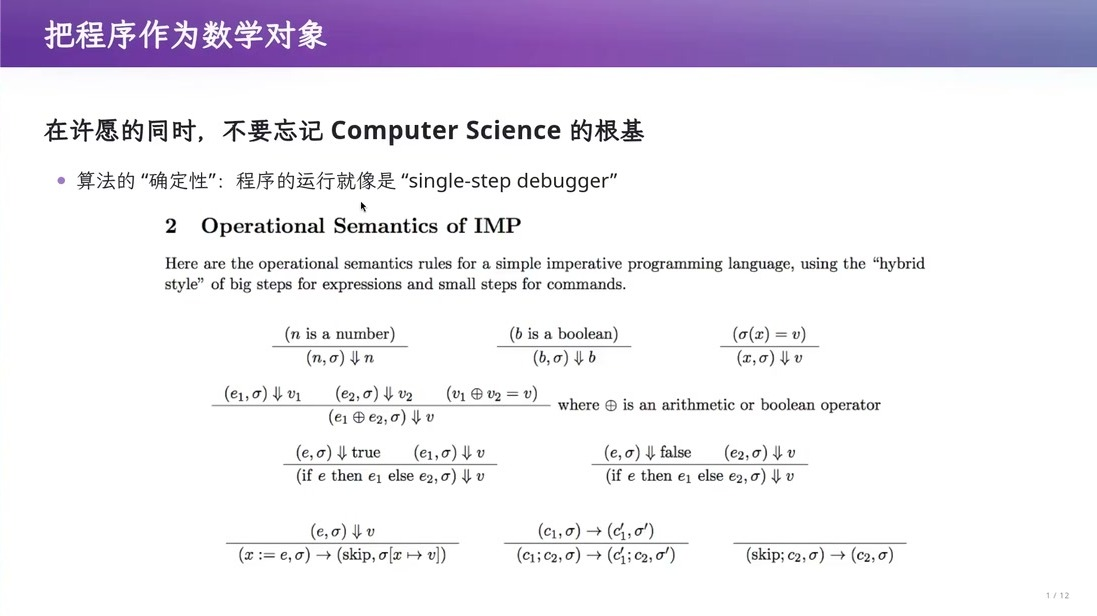
\includegraphics[width=0.88\textwidth]{figures/fig10_program_as_mathematical_object.jpg}
\caption{把程序作为数学对象：简单命令式语言 IMP 的操作语义（Operational Semantics）推理规则——程序的运行就是单步调试器上的状态演进\vtag}
\label{fig:fig10_program_as_mathematical_object}
\end{figure}
\srcnote{00:15:50--00:18:15}

如对应配图所示，在程序设计语言理论中，我们用 $\sigma : \mathit{Var} \to \mathbb{Z}$ 表示程序的当前存储器状态（State，即变量名到数值的映射）。对于算术/布尔表达式 $e$，采用大步求值语义（Big-step Semantics）记号 $\langle e, \sigma \rangle \Downarrow v$ 表示在状态 $\sigma$ 下表达式 $e$ 求值得到常量 $v$：
\begin{equation}
\frac{}{\langle n, \sigma \rangle \Downarrow n} \;(\text{Num}), \qquad
\frac{(\sigma(x) = v)}{\langle x, \sigma \rangle \Downarrow v} \;(\text{Var}), \qquad
\frac{\langle e_1, \sigma \rangle \Downarrow v_1 \quad \langle e_2, \sigma \rangle \Downarrow v_2 \quad (v_1 \oplus v_2 = v)}{\langle e_1 \oplus e_2, \sigma \rangle \Downarrow v} \;(\text{Op})
\label{eq:imp_big_step_expr}
\end{equation}
而对于会修改状态的命令/语句（Commands $c$），则采用小步状态转移语义（Small-step Semantics）记号 $\langle c, \sigma \rangle \to \langle c', \sigma' \rangle$，精确刻画单步调试器（Single-step Debugger）每按一次 \texttt{Step Into} 时的状态跃迁：
\begin{equation}
\frac{\langle e, \sigma \rangle \Downarrow v}{\langle x := e, \sigma \rangle \to \langle \mathbf{skip}, \sigma[x \mapsto v] \rangle}, \quad
\frac{\langle c_1, \sigma \rangle \to \langle c_1', \sigma' \rangle}{\langle c_1; c_2, \sigma \rangle \to \langle c_1'; c_2, \sigma' \rangle}, \quad
\frac{}{\langle \mathbf{skip}; c_2, \sigma \rangle \to \langle c_2, \sigma \rangle}
\label{eq:imp_small_step_cmd}
\end{equation}
在公式 \eqref{eq:imp_small_step_cmd} 中，$\sigma[x \mapsto v]$ 表示将状态 $\sigma$ 中变量 $x$ 的绑定更新为 $v$、其余变量保持不变的新状态（对应配图）。正因为每一条语句都有如公式 \eqref{eq:imp_big_step_expr}--\eqref{eq:imp_small_step_cmd} 般严丝合缝的数学定义，我们才能从测试（Testing）、分析（Analysis）与验证（Verification）三个不同维度对程序展开科学研究。

\begin{figure}[H]
\centering

\includegraphics[width=0.72\textwidth]{figures/fig11_board_state_transition_graph.jpg}
\caption{黑板板书：从初始状态出发，程序单步执行 $\sigma \to \sigma'$ 构成的确定性转移链与外部输入引发的树状分支\vtag}
\label{fig:fig11_board_state_transition_graph}
\end{figure}
\srcnote{00:16:40--00:18:10}

\subsection{方向一：软件测试（Testing）、Oracle 与编译器覆盖率插桩机制}

利用程序数学语义的第一种方式是\textbf{软件测试（Software Testing）}（对应配图）：不在抽象符号上做推导，而是直接从庞大的输入空间 $\mathcal{X}$ 中选定一组具体输入 $X_{\text{sel}} = \{x_1, x_2, \dots, x_k\} \subset \mathcal{X}$，在真实或模拟环境中运行被测程序 $P(x_i)$ 得到实际输出，再将其与预期结果或应当满足的性质——即\textbf{测试神谕（Test Oracle）}——进行比对。

\begin{figure}[H]
\centering
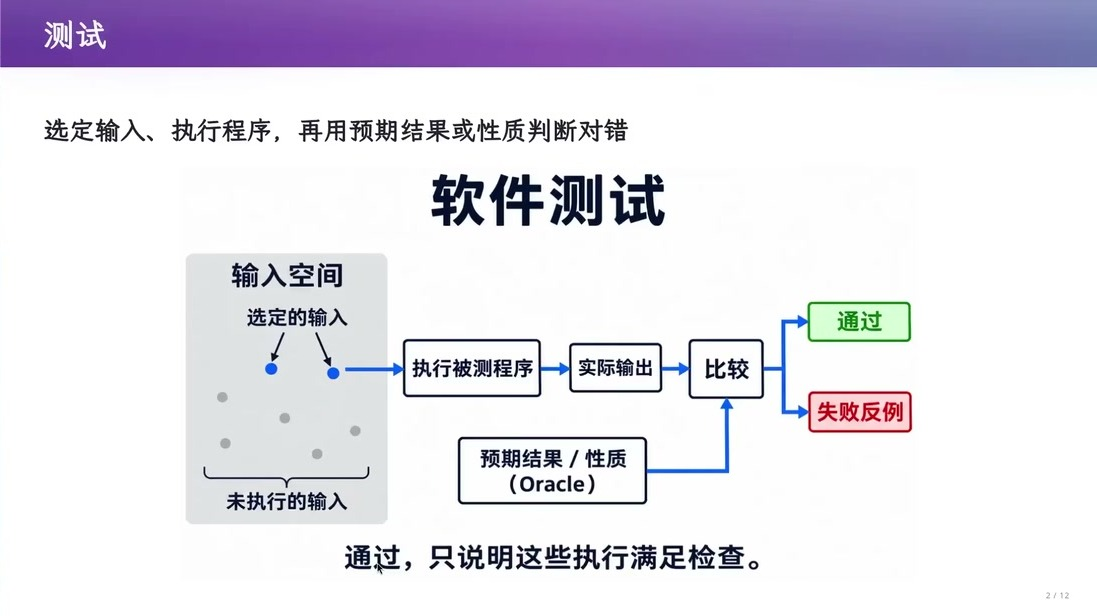
\includegraphics[width=0.88\textwidth]{figures/fig12_software_testing_oracle_flow.jpg}
\caption{软件测试原理框图：从输入空间选定离散输入执行被测程序，通过预期结果/性质（Oracle）判定通过或产出失败反例\vtag}
\label{fig:fig12_software_testing_oracle_flow}
\end{figure}
\srcnote{00:18:20--00:22:00}

测试的最大特点是“具体且直接”，但它的局限也一目了然：测试通过，仅仅证明了程序在你选定的那有限几个离散点 $X_{\text{sel}}$ 上满足检查，而输入空间里剩下广袤的未执行区域依然是未知的盲区（对应配图）。

\begin{figure}[H]
\centering
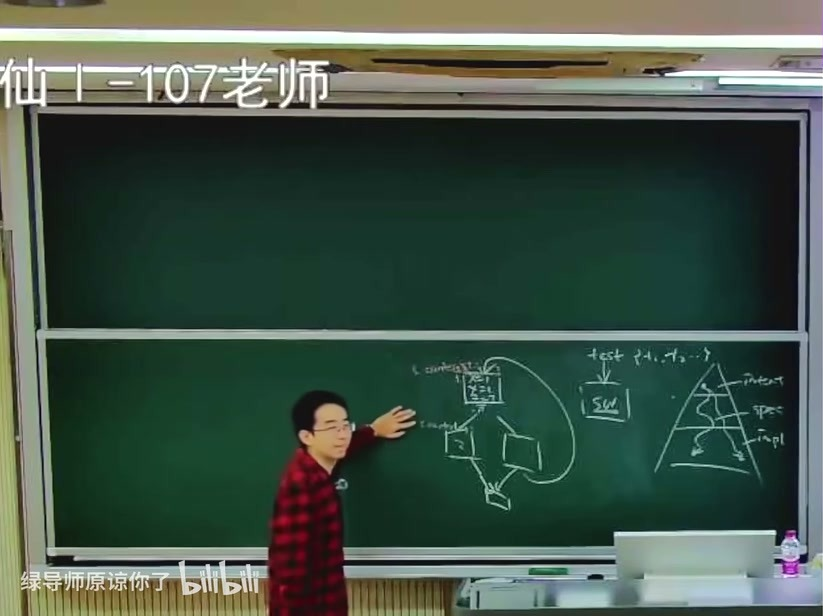
\includegraphics[width=0.72\textwidth]{figures/fig13_board_input_space_sampling.jpg}
\caption{黑板板书：左侧展示控制流基本块（Basic Block）拆分与插桩计数，右侧展示输入空间中的测试采样与未覆盖区域\vtag}
\label{fig:fig13_board_input_space_sampling}
\end{figure}
\srcnote{00:22:05--00:24:30}

那么，既然测试不能穷尽输入空间，软件工程师如何评估一组测试用例 $X_{\text{sel}}$ 到底够不够好？这就引出了经典的工程门禁指标——\textbf{代码覆盖率（Code Coverage）}。在工程实践中，我们完全可以向 AI Agent 许愿配置一条铁腕 CI 门禁：“如果单元测试的代码覆盖率到不了 \textbf{100\%}，就直接拒绝合并！”一旦门禁建立，当覆盖率到不了 \textbf{100\%} 时，Agent 就会根据未覆盖行号自动补充单元测试，直到达成 \textbf{100\%} 覆盖率。

主讲教师在这里追问了一个极具启发性的底层机制问题：\textbf{你每天都在看测试覆盖率报告，但你有没有想过，工具究竟是怎么算出一份代码有没有达到 100\% 覆盖率的？}
\begin{itemize}
    \item \textbf{笨办法（调试器单步跟踪）}：用 GDB 启动程序，每执行一步指令就读取当前行号并记录下来。这虽然概念上可行，但每次单步陷入内核（\texttt{ptrace}）会让程序慢上成千上万倍。
    \item \textbf{聪明的办法（编译器控制流图基本块插桩，Compiler Instrumentation）}：编译器在将源代码翻译为中间表示时，会自然构建出程序的\textbf{控制流图（Control Flow Graph，CFG）} $G = (V, E)$。其中每个节点 $B_i \in V$ 是一个\textbf{基本块（Basic Block）}——即一段“只有一个入口、只有一个出口、中间没有任何分支跳转”的连续顺序指令序列（如 `\texttt{x = 1; y = 2; z = 3;}`）。只要程序进入了基本块 $B_i$ 的第一条指令，该基本块内的所有指令就必定会顺序执行到底！
    因此，当我们在编译时开启覆盖率插桩选项（如 `\texttt{gcc --coverage}` 或 `\texttt{rustc -C instrument-coverage}`），编译器只需在每个基本块 $B_i$ 的入口处自动插入一条极轻量的计数指令 `\texttt{counter[i]++}`。在现代超标量乱序执行（Out-of-Order Execution）CPU 上，这条顺序追加的加法指令几乎可以被指令级并行（ILP）流水线完全隐藏延迟。运行完测试集后，工具只需扫描数组 $\mathit{counter}[1\dots |V|]$，即可精确计算出基本块/语句覆盖率：
    \begin{equation}
    \mathrm{Coverage}_{\text{BB}}(X_{\text{sel}}) \;=\; \frac{\big|\{ B_i \in V \mid \mathit{counter}[i] > 0 \}\big|}{|V|} \times 100\%
    \label{eq:basic_block_coverage}
    \end{equation}
\end{itemize}

\begin{knowledgebox}{工程启示：每一项看似理所当然的指标背后，都是精巧的底层机制（Mechanism）}
今天我们可以轻描淡写地要求 Coding Agent 把单元测试覆盖率刷到 \textbf{100\%}，甚至利用 Intel PT（Processor Trace）等硬件特性零开销采集分支轨迹；但这背后依靠的是几代编译器与系统工程师打造的 CFG 基本块插桩机制（公式 \eqref{eq:basic_block_coverage}）。工具把复杂的动态执行浓缩成了“哪几行代码计数仍为 $0$”的清晰反馈信号，才让人类和 AI 拥有了持续改进测试的抓手。
\end{knowledgebox}

% =========================================================================
% SECTION 3
% =========================================================================
\section{程序分析、形式化验证与 Rice 定理的不可判定性铁幕}

\subsection{方向二：程序分析（Program Analysis）与区间抽象解释}

如果我们不想一个一个输入去跑测试，能不能把成千上万个具体状态“捆绑打包”成一个\textbf{抽象状态（Abstract State）}，直接在抽象状态上模拟运行程序，从而一次性推导出所有可能执行的行为边界？这就是\textbf{程序分析（Program Analysis）}与\textbf{抽象解释（Abstract Interpretation，Cousot \& Cousot 1977）}的核心思想（对应配图）。

\begin{figure}[H]
\centering
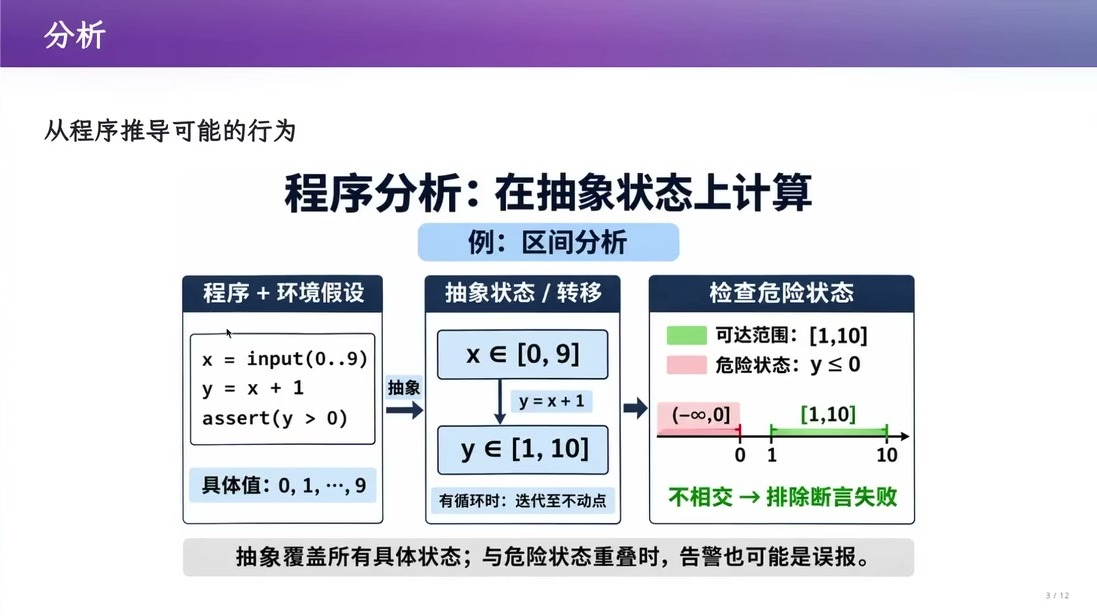
\includegraphics[width=0.88\textwidth]{figures/fig14_abstract_interpretation_interval.jpg}
\caption{程序分析——在抽象状态上计算：以区间分析（Interval Analysis）推导 $x \in [0,9] \xrightarrow{y = x+1} y \in [1,10]$ 与危险状态 $(-\infty, 0]$ 不相交为例\vtag}
\label{fig:fig14_abstract_interpretation_interval}
\end{figure}
\srcnote{00:24:35--00:29:30}

考察对应配图中的三行代码：
\begin{lstlisting}[language=Python, caption={区间抽象解释示例程序}]
x = input(0..9)   # 环境假设：外部输入 x 取值于具体集合 {0, 1, ..., 9}
y = x + 1
assert(y > 0)
\end{lstlisting}
在具体语义下，读入 `x` 会让状态树瞬间分叉出 $10$ 个分支（若读入 64 位整数则分叉出 $2^{64}$ 个分支，对应配图）。而在\textbf{区间抽象域（Interval Domain）} $\mathcal{I} = \{[l, u] \mid l, u \in \mathbb{Z} \cup \{-\infty, +\infty\},\; l \le u\} \cup \{\bot\}$ 上，我们不再逐个枚举具体数值，而是只跟踪每个变量的上下界区间：
\begin{equation}
\begin{aligned}
&\text{1. 初始抽象状态：} && x^\# = [0, 9] \\
&\text{2. 抽象转移算子 }\texttt{y = x + 1}\text{：} && y^\# = x^\# +^\# [1, 1] = [0 + 1,\, 9 + 1] = [1, 10] \\
&\text{3. 危险状态交集检查：} && \text{Bad} = \{y \in \mathbb{Z} \mid y \le 0\} = (-\infty, 0], \quad y^\# \cap \text{Bad} = [1, 10] \cap (-\infty, 0] = \emptyset
\end{aligned}
\label{eq:interval_abstract_interpretation}
\end{equation}

\begin{figure}[H]
\centering
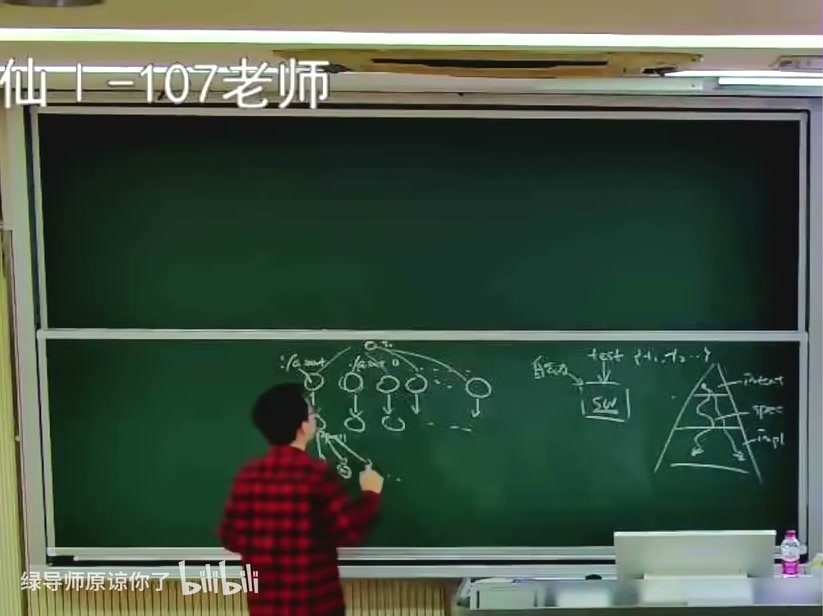
\includegraphics[width=0.72\textwidth]{figures/fig15_board_concrete_vs_abstract_tree.jpg}
\caption{黑板板书：从初始命令行参数 \texttt{argc/argv} 与 \texttt{input} 引发的具体状态树指数分叉，到捆绑合并为单一抽象状态的演化\vtag}
\label{fig:fig15_board_concrete_vs_abstract_tree}
\end{figure}
\srcnote{00:25:30--00:28:40}

一般地，设具体程序所有真实可达状态的集合为 $R_{\text{conc}}$，健全（Sound）的抽象解释通过拓宽算子（Widening Operator，用于在循环中加速收敛到不动点）计算出一个包含所有真实可达状态的\textbf{过近似集合（Over-approximation）} $R^\#_{\text{abs}}$：
\begin{equation}
R_{\text{conc}} \;\subseteq\; \gamma(R^\#_{\text{abs}})
\qquad \Longrightarrow \qquad
\Big(\gamma(R^\#_{\text{abs}}) \cap \text{Bad} = \emptyset \implies R_{\text{conc}} \cap \text{Bad} = \emptyset\Big)
\label{eq:sound_over_approximation}
\end{equation}
如公式 \eqref{eq:sound_over_approximation} 所示：因为抽象状态覆盖了全部具体状态，只要抽象可达集 $\gamma(R^\#_{\text{abs}})$ 与危险状态集 $\text{Bad}$ 不相交（如 $[1, 10] \cap (-\infty, 0] = \emptyset$），就能给出百分之百的数学安全保证（排除断言失败）！但反过来，如果 $\gamma(R^\#_{\text{abs}}) \cap \text{Bad} \neq \emptyset$，则既可能是程序真的有 Bug，也可能仅仅是因为抽象区间放得太宽（丢掉了变量间的关联精度）而把实际不可达的坏状态算了进去——这就是静态分析著名的\textbf{误报（False Positive）}来源。\begin{warningbox}{静态分析的固有边界：为什么健全性（Soundness）往往伴随着误报（False Positive）？}
根据公式 \eqref{eq:sound_over_approximation}，健全的抽象解释为了保证“绝不漏掉任何真实可达状态（$R_{\text{conc}} \subseteq \gamma(R^\#_{\text{abs}})$）”，必须在遇到分支合并与循环时采取保守的过近似（Over-approximation）。当抽象域丢掉了变量之间的耦合关系（例如忘了 $x$ 与 $y$ 恒相等）或遇到指针别名、内联汇编、系统调用时，抽象状态集合就会膨胀并触碰危险区域 $\text{Bad}$，从而产生大量令开发者头疼的静态误报。
\end{warningbox}

而在真实工业语言（如 C/C++）中，一旦遇到复杂的函数指针、内联汇编（Inline Assembly）或操作系统调用（System Call），精确建模抽象转移函数的难度就会急剧上升。

\subsection{方向三：程序验证（Program Verification）与证明义务}

第三种方式就是我们在第 12 讲深入讨论过的\textbf{程序验证（Program Verification）}（对应配图）：将规格说明（Specification）、环境假设与程序源码一起送入验证条件生成器（VCGen），转化为纯粹的数学\textbf{证明义务（Proof Obligations）}（如 Hoare 三元组 $\{x \ge 0\}\; x := x + 1\; \{x > 0\}$），交由自动定理证明器（SMT Solver）或交互式证明助手（Lean / Coq）裁决。

\begin{figure}[H]
\centering
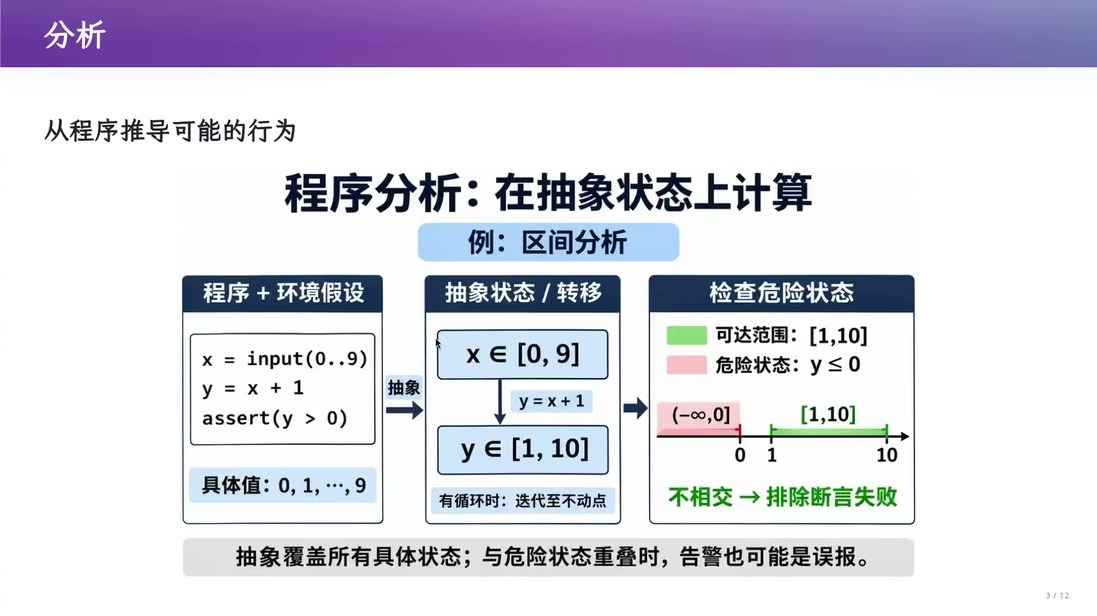
\includegraphics[width=0.88\textwidth]{figures/fig16_program_verification_obligations.jpg}
\caption{程序验证原理框图：将规格、环境假设与程序/模型转化为证明义务，验证器输出“已证明”“反例轨迹”或“unknown（未知）”\vtag}
\label{fig:fig16_program_verification_obligations}
\end{figure}
\srcnote{00:29:35--00:29:58}

特别注意对应配图右侧的三种输出状态：除了“已证明（Proved）”和“反例（Counterexample）”之外，验证器还经常会输出第三种结果——\textbf{\texttt{unknown}（无法完成证明）}！理解 \texttt{unknown} 极其关键：验证器给出 \texttt{unknown}（或证明助手里卡住证不下去），\textbf{绝不等于程序一定有 Bug}；它很可能只是因为求解器超时、缺少一条关键的辅助归纳引理（Lemma），或者环境模型假设还不够精细。

\subsection{Rice 定理（1953）与嵌入费马大定理的 4 行代码：为什么没有万能分析器？}

既然程序是严格的数学对象，我们能不能一劳永逸地发明一个“万能程序验证/分析算法”，输入任意一段程序 $P$，就能自动判断它会不会崩溃、会不会触发 `\texttt{abort()}`？

1953 年，Henry Gordon Rice 证明了可计算性理论中最具统治力的不可能定理之一——\textbf{Rice 定理（Rice's Theorem）}，彻底击碎了这一幻想（对应配图）：

\begin{figure}[H]
\centering
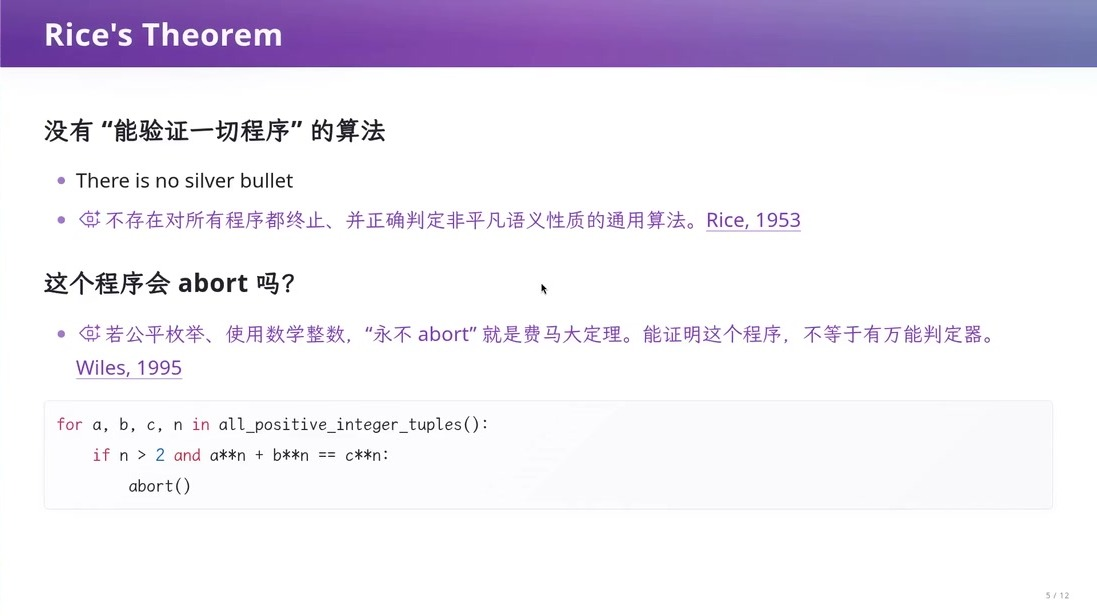
\includegraphics[width=0.88\textwidth]{figures/fig17_rices_theorem_fermat.jpg}
\caption{Rice's Theorem（1953）：不存在对所有程序都终止且正确判定非平凡语义性质的通用算法，以及将费马大定理（Wiles, 1995）嵌入其中的 4 行代码\vtag}
\label{fig:fig17_rices_theorem_fermat}
\end{figure}
\srcnote{00:30:00--00:35:00}

\begin{importantbox}{定理陈述：Rice 定理（Rice's Theorem, 1953）}
设 $\mathcal{P}$ 为图灵完备编程语言中所有程序构成的集合，$\mathcal{S}$ 为程序语义行为（即程序所计算的部分函数 $[\![ P ]\!]$）的集合。对于任意一个关于程序语义的性质 $\Phi \subseteq \mathcal{S}$，只要 $\Phi$ 是\textbf{非平凡的（Non-trivial）}——即既存在满足 $\Phi$ 的程序，也存在不满足 $\Phi$ 的程序（$\Phi \neq \emptyset$ 且 $\Phi \neq \mathcal{S}$）——那么判定任意给定程序 $P$ 的语义是否满足 $\Phi$ 的问题：
\begin{equation}
L_{\Phi} \;=\; \big\{\, P \in \mathcal{P} \;\big|\; [\![ P ]\!] \in \Phi \,\big\}
\label{eq:rices_theorem_language}
\end{equation}
在数学上是\textbf{严格不可判定的（Undecidable）}！换言之，宇宙间绝不存在一个算法 $\mathcal{A} : \mathcal{P} \to \{\mathsf{True}, \mathsf{False}\}$，能够对所有输入程序 $P$ 在有限时间内停机，并百分之百正确地回答 $[\![ P ]\!] \in \Phi$ 是否成立。
\end{importantbox}

为什么哪怕是判断“这个程序会不会执行 `\texttt{abort()}`（或会不会解引用空指针）”这样看似简单的语义性质，在一般意义下都不可判定？主讲教师没有用枯燥的对角线停机问题规约，而是给出了对应配图中一段令人拍案叫绝的 **4 行 Python 程序**：

\begin{lstlisting}[language=Python, caption={将费马大定理（Fermat's Last Theorem）编码为程序是否执行 \texttt{abort()} 的判定问题}]
for a, b, c, n in all_positive_integer_tuples():
    if n > 2 and a**n + b**n == c**n:
        abort()
\end{lstlisting}

在黑板上，主讲教师演示了如何用几行协程生成器 `\texttt{yield}` 轻松写出一个公平枚举所有正整数四元组 $(a, b, c, n) \in (\mathbb{Z}^+)^4$ 的枚举器 `\texttt{all\_positive\_integer\_tuples()}`（例如按和 $S = a + b + c + n = 4, 5, 6, \dots$ 分层遍历）。假设该程序运行在理想数学整数（Python 原生支持任意精度大整数）和无限内存上，那么请问：\textbf{上面这 4 行程序在运行过程中永远不会触发 \texttt{abort()} 吗？}

写成数学公式，这段程序永不执行 `\texttt{abort()}` 的充要条件恰好就是困扰了人类数学界三百五十余年、直到 1995 年才由 Andrew Wiles 动用模形式与椭圆曲线谷山--志村猜想写成上百页天书证明的\textbf{费马大定理（Fermat's Last Theorem）}：
\begin{equation}
\text{Program never calls }\texttt{abort()} \quad \Longleftrightarrow \quad \forall a, b, c, n \in \mathbb{Z}^+:\; \big(n > 2 \implies a^n + b^n \neq c^n\big)
\label{eq:fermat_last_theorem_abort}
\end{equation}
如果世界上真的存在一个“能自动判断任意程序会不会 `\texttt{abort()}`（或会不会在 `\texttt{abort()}` 处发生空指针解引用）”的万能静态分析器，那么我们只需要把上面这 4 行代码（或者把条件换成哥德巴赫猜想、孪生素数猜想、黎曼猜想的反例枚举）喂给这个分析器，它一秒钟就能替全人类解决所有未解的数论难题！这显然是不可能的。

\begin{figure}[H]
\centering
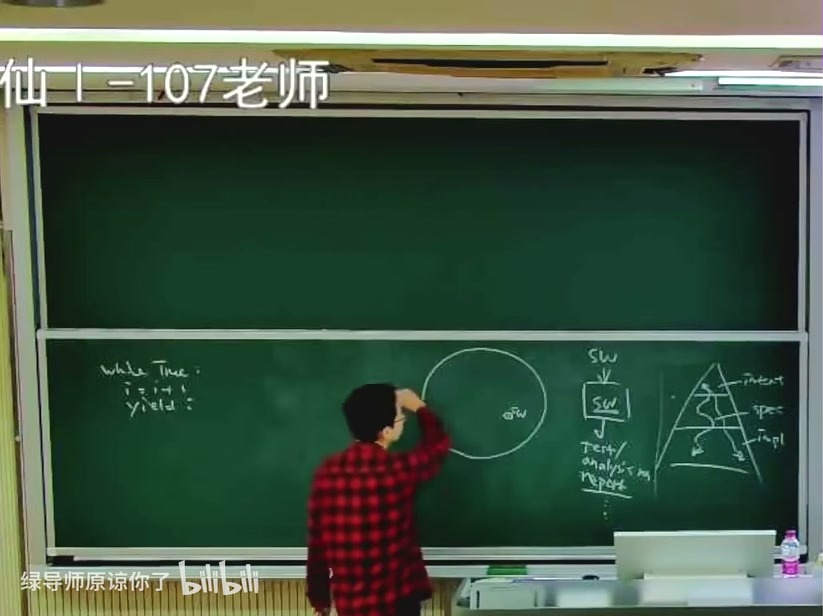
\includegraphics[width=0.72\textwidth]{figures/fig18_board_undecidability_set_boundary.jpg}
\caption{黑板板书：左侧展示枚举正整数元组的生成器 `\texttt{while True: ... yield}`，右侧展示所有可能程序空间 $\mathcal{P}_{\text{all}}$ 中人类真实工程程序 $\mathcal{P}_{\text{human}}$ 仅占极小一角\vtag}
\label{fig:fig18_board_undecidability_set_boundary}
\end{figure}
\srcnote{00:35:05--00:37:50}

然而，既然 Rice 定理给“万能程序分析器”判了死刑，为什么软件分析工具在现实工业界依然大放异彩？主讲教师在黑板上画了一个大圆套小圆的集合图（对应配图右侧），道破了理论与工程之间的关键差异：
\begin{itemize}
    \item \textbf{人类真实编写的软件只是所有可能程序空间中的极小良构子集（$\mathcal{P}_{\text{human}} \ll \mathcal{P}_{\text{all}}$）}：没有任何一个正常的软件工程师会在写支付宝下单逻辑或教务选课系统时，在 `\texttt{if}` 条件里塞进一个费马大定理或哥德巴赫猜想的枚举器！真实的业务软件是人类物理世界过程在信息世界的投影，往往遵循固定的信息系统范式（用关系数据库存储状态、用标准事务迁移状态）。
    \item \textbf{缺陷预测（Defect Prediction）的启发式威力}：正因为人类写出的代码带有强烈的规律性，哪怕是最粗糙的统计启发式方法也能奏效。例如早年软件工程界流行的缺陷预测研究：根本不看程序的执行语义，仅仅通过统计一个类（Class）里有多少个 `\texttt{int}` 关键字、多少个循环、最大大括号嵌套深度是多少，拼成一个上千维的特征向量 $\vec{x} \in \mathbb{R}^d$ 送入分类器 $F(\vec{x})$，就能给出诸如“我有 \textbf{99.9\%} 的把握认为这段代码里有 Bug”的预测——而且在真实老旧项目上往往还真能猜中风险最高的模块！
\end{itemize}

因此，面对不可判定性的铁幕，软件工程给出的回答无比务实：\textbf{既然没有银弹，那就做取舍（Let's Trade Off）！}任何实用的软件分析工具，必然在\textbf{健全性（Soundness，无漏报）}、\textbf{完备性（Completeness，无误报）}与\textbf{可终止性/效率（Termination \& Efficiency）}的不可能三角中做出妥协：
\begin{equation}
\begin{cases}
\textbf{Soundness（健全性）：} & \text{Tool says Safe} \implies \text{Truly Safe（无漏报 FN）} \\[4pt]
\textbf{Completeness（完备性）：} & \text{Truly Safe} \implies \text{Tool says Safe（无误报 FP）}
\end{cases}
\label{eq:soundness_completeness_tradeoff}
\end{equation}

% =========================================================================
% SECTION 4
% =========================================================================
\section{Let's Trade Off（一）：静态分析工具的取舍（类型系统、Linter 与抽象解释）}

为了看清每一种经典软件分析工具究竟在公式 \eqref{eq:soundness_completeness_tradeoff} 的权衡中“保留了什么抽象、忘掉了什么细节、从哪里获取项目知识”，主讲教师首先梳理了三大\textbf{静态分析（Static Analysis）}工具的取舍矩阵（对应配图与对应汇总表）：

\begin{figure}[H]
\centering
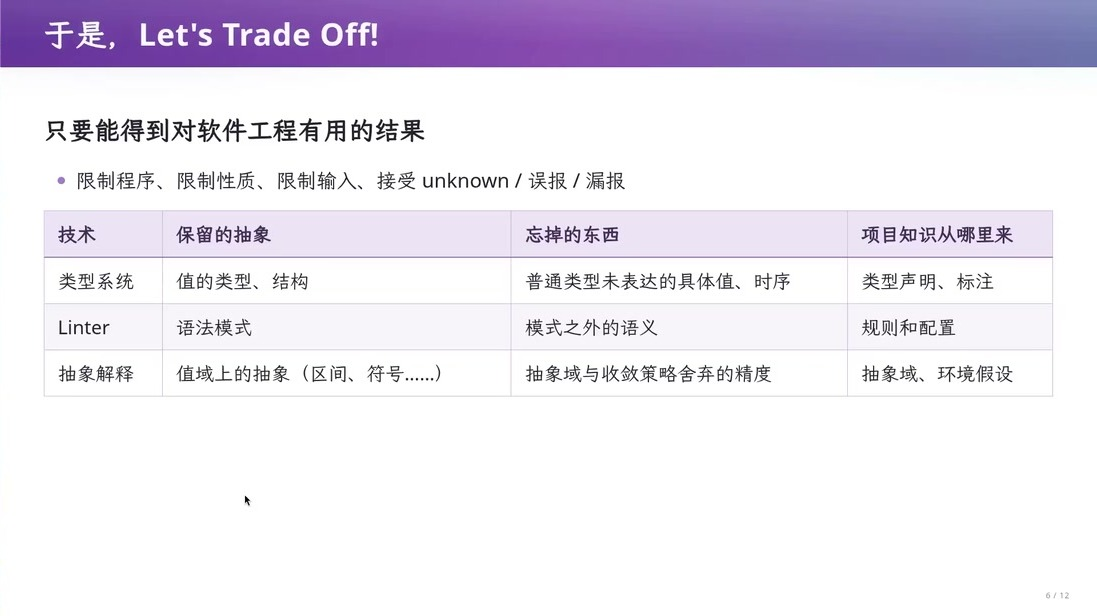
\includegraphics[width=0.88\textwidth]{figures/fig19_static_analysis_tradeoff_table.jpg}
\caption{于是，Let's Trade Off（静态分析篇）：类型系统、Linter 与抽象解释在保留抽象、遗忘细节与知识来源上的三维对比\vtag}
\label{fig:fig19_static_analysis_tradeoff_table}
\end{figure}
\srcnote{00:37:55--00:38:45}

\begin{table}[H]
\centering
\caption{静态分析工具的三维取舍矩阵（保留的抽象 vs. 忘掉的东西 vs. 知识来源）}
\label{tab:static_tradeoff_matrix}
\begin{tabular}{p{2.2cm}p{3.4cm}p{4.0cm}p{3.3cm}}
\toprule
\textbf{技术名称} & \textbf{保留的抽象（Retained）} & \textbf{忘掉的东西（Forgotten）} & \textbf{项目知识从哪里来} \\
\midrule
类型系统 & 值的类型、代数结构、所有权生命周期 & 普通类型未表达的具体数值、调用时序、业务规则 & 程序员编写的类型声明与类型标注 \\
Linter & 语法树（AST）模式、局部控制流与数据流结构 & 模式之外的深层运行时语义与跨模块动态行为 & 团队编码规范与配置文件（Rules） \\
抽象解释 & 值域上的数学抽象（区间、正负号、多面体等） & 抽象域与拓宽收敛策略故意忽略的具体数值精度 & 抽象域设计、转移函数与环境假设 \\
\bottomrule
\end{tabular}
\end{table}

\subsection{类型系统（Type System）：从 JavaScript 隐式转换乱象到 Rust 编译期博弈}

类型系统是人类发明的最成功、使用最广泛的轻量级形式化方法：它彻底“忘掉”了变量在运行时的具体数值（比如把 `$0$`、`$1$`、`$-99$` 统统折叠抽象为同一个类型符号 `\texttt{int}`），从而得以在编译期以线性或近线性时间静态排除一整类非法操作。

如果一门语言缺乏严格的类型系统、甚至允许随心所欲的隐式类型转换（Implicit Type Coercion），会发生什么灾难？主讲教师展示了前端界广为流传的“圣三位一体（Holy Trinity）”与 **JavaScript 弱类型相等性（\texttt{==}）反面教材**（对应配图）：

\begin{figure}[H]
\centering
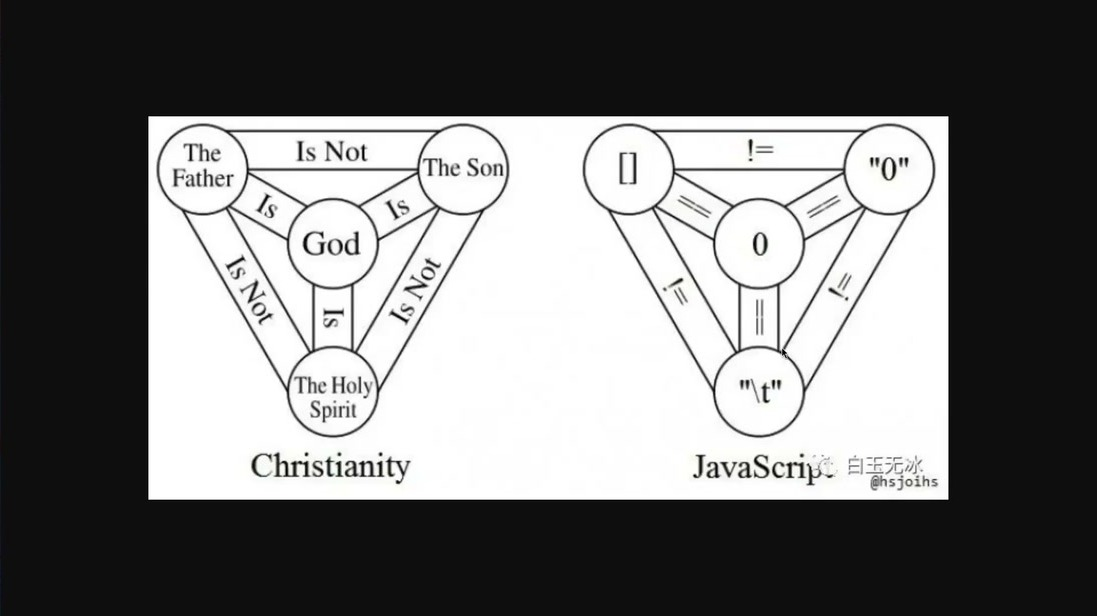
\includegraphics[width=0.78\textwidth]{figures/fig20_holy_trinity_js_type_meme.jpg}
\caption{类型系统的反面教材：对比基督教三位一体图与 JavaScript 弱类型隐式转换下 `\texttt{0}`、`\texttt{"0"}`、`\texttt{[]}`、`\texttt{"\textbackslash t"}` 违背等价关系传递性的乱象\vtag}
\label{fig:fig20_holy_trinity_js_type_meme}
\end{figure}
\srcnote{00:38:50--00:40:20}

在离散数学中，任何合理的相等关系（Equivalence Relation）都必须满足自反性、对称性与\textbf{传递性（Transitivity：$a = b \land b = c \implies a = c$）}。但在 JavaScript 的松散相等运算符 `\texttt{==}` 下，由于存在把空数组 `\texttt{[]}` 和空白字符串 `\texttt{"\textbackslash t"}` 隐式转换为数字 `\texttt{0}` 的奇葩规则，竟然同时成立以下违背传递性的荒诞关系：
\begin{equation}
\begin{aligned}
\texttt{0 == "0"} \quad (\mathsf{true}), \qquad
&\texttt{0 == []} \quad (\mathsf{true}), \qquad
\texttt{0 == "\textbackslash t"} \quad (\mathsf{true}) \\
\text{但两两之间却全部不等：}\quad
&\texttt{"0" == []} \quad (\mathsf{false}), \qquad
\texttt{[] == "\textbackslash t"} \quad (\mathsf{false}), \qquad
\texttt{"0" == "\textbackslash t"} \quad (\mathsf{false})
\end{aligned}
\label{eq:js_non_transitive_equality}
\end{equation}
正因为在弱类型动态语言里吃够了运行时莫名其妙卡死或算出 `\texttt{NaN}` 的苦头，现代软件工程全面转向强静态类型系统（如 TypeScript、Rust、现代 C++）。

强类型系统的代价是什么？是\textbf{将证明成本转嫁给了写代码的程序员（或 Coding Agent）}：
\begin{itemize}
    \item 在早期 C++ 中，即便编译器明明知道元组解包的类型，程序员也必须手写冗长的类型声明，直到 C++17 引入结构化绑定（`\texttt{auto [a, b] = ...}`）才得以简化；
    \item 而在 \textbf{Rust} 中，为了在编译期静态保证内存安全与无数据竞争，借用检查器（Borrow Checker）引入了所有权与生命周期类型系统。许多在 C 语言里完全合法、在运行时也确实不会出错的无环图或双向链表写法，因为超出了 Rust 静态类型系统的表达边界而直接被编译器拒绝（产生静态误报/保守拒绝）。程序员不得不大做“类型体操”来讨好编译器，但一旦编译通过，就买到了“绝无悬垂指针与并发数据竞争”的铁律保证。
\end{itemize}

\subsection{Linter 的二八定律：用确定性语法规则拦截 80\% 的低级缺陷}

有些代码完全符合编程语言的类型系统，甚至语法上百分之百合法，但在工程上却是极其危险的坏味道（Bad Smell）。例如在 C 语言中，语法允许你写下极其狂野的强制类型转换——你甚至可以把一个硬编码的十六进制整数地址（包含前缀 \textbf{0x}，如 `\texttt{0x1234}`）直接强转为函数指针并调用它：
\begin{lstlisting}[language=C, caption={C 语言中语法合法但工程上极度危险的硬编码地址函数指针强转}]
typedef void (*func_ptr_t)(void);
((func_ptr_t)0x1234)(); // 将立即数 0x1234 强转为函数指针直接跳转执行！
\end{lstlisting}
在编写底层固件或教学演示时，我们偶尔会故意写 `\texttt{0x1234}` 这样的底层黑魔法；但如果你开发的是要上火星的航天器控制软件（如 JPL / MISRA C 标准），任何未经严格审批的强制类型转换或超过 3 层的 `\texttt{if}` 嵌套都是绝对禁止的。

这类“编译器不管、但工程规范严禁”的检查，就交给了 \textbf{Linter}（如 \texttt{clang-tidy}、\texttt{clippy}、\texttt{eslint}、\texttt{ruff}）。在课堂终端演示中，主讲教师展示了一份总结得极为精辟的\textbf{“Linter 二八定律清单”}（对应配图）：

\begin{figure}[H]
\centering

\includegraphics[width=0.80\textwidth]{figures/fig21_linter_8020_categories_notes.jpg}
\caption{终端技术笔记：Linter 的黄金二八定律——只做能 100\% 判定的局部检查，覆盖最高 ROI 的六大缺陷类别\vtag}
\label{fig:fig21_linter_8020_categories_notes}
\end{figure}
\srcnote{00:42:30--00:44:30}

\begin{practicebox}{Linter 的设计黄金准则与六大高 ROI 检查类别}
如对应配图所示，优秀的 Linter 遵循一条清晰的边界准则：\textbf{Linter 只做局部能够 100\% 确定性判定的事；凡是依赖“大局观、跨模块业务语义”的判断，要么交给类型系统与契约测试，要么交给阅读代码的审查者，否则误报率一高，开发者就会把整个 Linter 关掉！}最高投资回报率（ROI）的六类 Linter 规则包括：
\begin{enumerate}
    \item \textbf{未使用 / 未定义 / 不可达（死代码）}：未使用的变量与 \texttt{import}、\texttt{return} 之后的死语句、恒真/恒假条件分支（常见于拷贝粘贴笔误或合并冲突残留，零误报）；
    \item \textbf{空安全与边界}：可能为 \texttt{null}/\texttt{undefined} 的解引用、数组越界访问、\texttt{switch} 缺少 \texttt{default}/穷尽分支、滥用非空断言（相当于“编译器帮不上的地方由 Linter 兜底防 Segfault”）；
    \item \textbf{异步与资源生命周期}：忘记 \texttt{await} 导致悬空的 \texttt{Promise}、\texttt{async} 函数漏写异常捕获、文件句柄/锁/数据库连接忘记 \texttt{close()}/\texttt{release()}、React \texttt{useEffect} 缺失依赖项；
    \item \textbf{危险 API 与隐式转换}：禁用 \texttt{eval}、禁用 TypeScript \texttt{any}、禁止字符串拼接 SQL、调用 \texttt{parseInt} 漏传进制基数 \texttt{radix}、浮点数直接用 \texttt{==} 比较；
    \item \textbf{依赖与架构约束（对 Agent 尤具价值）}：检测循环依赖、禁止跨架构分层违规引用（如禁止 UI 层直接 \texttt{import} 数据库底层模块）——\textbf{这类架构边界规则是大语言模型最容易退化破坏的地方，也是唯一靠人眼 Code Review 极难逐一盯防的地方}；
    \item \textbf{可维护性阈值}：圈复杂度（Cyclomatic Complexity）过高、函数过长、参数过多、嵌套过深。
\end{enumerate}
\end{practicebox}

% =========================================================================
% SECTION 5
% =========================================================================
\section{Let's Trade Off（二）：动态执行与形式化模型取舍及强化学习反馈飞轮}

\subsection{在执行中取舍：Fuzzing、Property-Based Testing 与差分/蜕变测试}

静态分析工具不运行程序，因此在面对动态输入与复杂运行时状态时不可避免地会丢失精度。而\textbf{动态执行类工具（Dynamic Execution Tools）}则做出了截然相反的取舍：它们放弃了对所有路径的静态覆盖，换取了在真实执行轨迹上百分之百准确的观测（对应配图与对应汇总表）。

\begin{figure}[H]
\centering
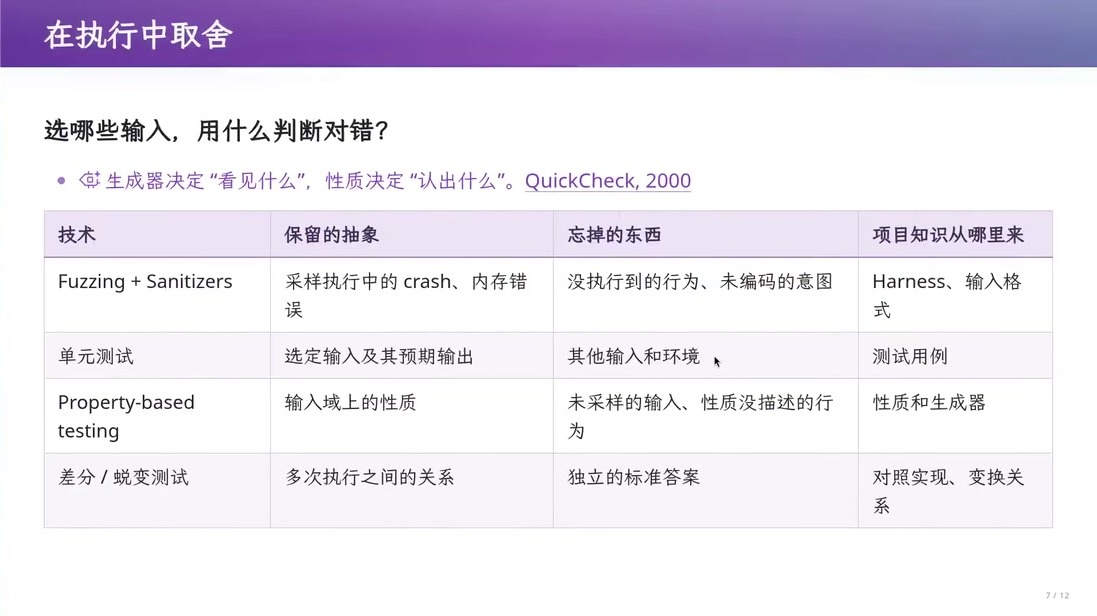
\includegraphics[width=0.88\textwidth]{figures/fig22_dynamic_execution_tradeoff_table.jpg}
\caption{在执行中取舍（动态工具篇）：Fuzzing+Sanitizers、单元测试、Property-based Testing（QuickCheck, 2000）与差分/蜕变测试的三维对比\vtag}
\label{fig:fig22_dynamic_execution_tradeoff_table}
\end{figure}
\srcnote{00:45:50--00:48:40}

\begin{table}[H]
\centering
\caption{动态执行与模型验证工具的三维取舍矩阵}
\label{tab:dynamic_model_tradeoff_matrix}
\begin{tabular}{p{2.5cm}p{3.3cm}p{3.8cm}p{3.3cm}}
\toprule
\textbf{技术名称} & \textbf{保留的抽象（Retained）} & \textbf{忘掉的东西（Forgotten）} & \textbf{项目知识从哪里来} \\
\midrule
Fuzzing + Sanitizers & 采样执行中的 Crash、内存越界与数据竞争 & 未执行到的代码分支、未编码为断言的业务意图 & 测试入口（Harness）与输入格式语法 \\
单元测试 & 选定离散输入点及对应的预期输出 & 选定输入点之外的输入空间与生产运行环境差异 & 开发者编写的具体测试用例（Test Cases） \\
Property-based Testing & 输入域与输出域之间的一般数学性质 & 未采样到的输入、性质未描述的其余行为 & 性质断言（Properties）与输入生成器（Generators） \\
差分 / 蜕变测试 & 多次执行结果之间的等价或变换关系 & 独立的绝对标准答案（Ground-truth Oracle） & 参考对照实现（Reference）或输入变换关系 \\
模型检验 & 有限状态机内的全部可达状态与时序性质 & 模型之外的外部世界与底层代码实现细节 & 人类专家编写的抽象状态机模型（如 TLA+） \\
符号执行 & 已探索路径上的精确分支路径约束 $\mathit{PC}$ & 未探索的循环/深层路径、被简化的外部系统环境 & 测试入口、符号变量声明与环境桩模型 \\
定理证明 & 形式化模型中的严密演绎逻辑性质 & 形式化规约与真实人类需求及真实运行环境间的 Gap & 形式化规格说明（Spec）与归纳证明脚本 \\
\bottomrule
\end{tabular}
\end{table}

在对应配图的四类动态测试范式中，有两项高级测试思想尤为值得深入掌握：
\begin{enumerate}
    \item \textbf{基于性质的测试（Property-Based Testing，Koen Claessen \& John Hughes, ICFP 2000 QuickCheck）}：
    传统单元测试由程序员手写几组固定的输入输出对（如 `\texttt{assert(sort([3,1,2]) == [1,2,3])}`）；而 Property-based Testing（如 Haskell 的 \texttt{QuickCheck}、Python 的 \texttt{Hypothesis}、Rust 的 \texttt{proptest}）则将注意力转移到了\textbf{对任意合法输入 $x \in \mathcal{D}$ 都应当恒成立的一般代数性质 $P(x)$} 上，例如：
    \begin{equation}
    \forall x \in \mathcal{D}_{\text{valid}}:\quad \mathrm{decode}\big(\mathrm{encode}(x)\big) = x
    \label{eq:property_based_roundtrip}
    \end{equation}
    这里的核心口诀是：\textbf{生成器（Generator）决定了测试能“看见什么”，性质（Property）决定了测试能“认出什么”}。\begin{knowledgebox}{QuickCheck 与蜕变测试的哲学：从“验证单点答案”跃迁到“验证代数不变量”}
无论是 Property-based Testing 中的编解码往返恒等式 $\mathrm{decode}(\mathrm{encode}(x)) = x$（公式 \eqref{eq:property_based_roundtrip}），还是蜕变测试中的奇函数性质 $\sin(-x) = -\sin(x)$（公式 \eqref{eq:metamorphic_testing_sin}），它们之所以能摆脱人类手写测试神谕（Oracle）的瓶颈，是因为它们将验证对象从“单个输入的绝对输出值”提升到了“多个输入输出之间的代数同态或对称关系”，从而解锁了无穷输入空间上的自动化随机探索。
\end{knowledgebox}

更精妙的是，一旦随机生成的某个复杂输入 $x_{\text{fail}}$ 触发了性质失败，QuickCheck 会自动启动\textbf{反例约简（Shrinking）}算法，在保持失败的前提下不断删减输入元素，最终留给开发者一个极简、极易调试的最小反例！
    \item \textbf{差分测试（Differential Testing）与蜕变测试（Metamorphic Testing）——当标准答案（Oracle）不存在时怎么办？}：
    对于编译器、模拟器或超越函数库，给定一个复杂输入 $x$，人类根本算不出它的标准答案 $y^*$ 是多少（即面临 \textbf{Oracle Problem}）。此时有两种破局之道：
    \begin{itemize}
        \item \textbf{差分测试}：准备两个或多个独立实现 $f_1, f_2$（如第 11 讲中的 NEMU 与 QEMU/Spike），对同一输入检验 $f_1(x) = f_2(x)$；
        \item \textbf{蜕变测试}：即便手里只有一个实现 $f$，也可以利用领域数学定律，对输入 $x$ 施加一个已知变换 $T_{\text{in}}(x)$，并检验两次运行输出是否满足对应的蜕变关系（Metamorphic Relation，$R_{\text{out}}$）：
        \begin{equation}
        \forall x \in \mathbb{R}:\quad f(-x) = -f(x) \quad (\text{以正弦函数 } f(x) = \sin(x) \text{ 的奇函数性质为例})
        \label{eq:metamorphic_testing_sin}
        \end{equation}
        比如你不知道 $\sin(1.234567)$ 精确到小数点后第 15 位到底是多少，但只要程序算出的 $\sin(-1.234567)$ 不等于 $-\sin(1.234567)$，或者 $\sin^2(x) + \cos^2(x) \neq 1$，就能立刻断定实现存在 Bug！
    \end{itemize}
\end{enumerate}

\subsection{在模型中取舍与“Pass 买到什么，Fail 留下什么？”}

同样地，哪怕是模型检验、符号执行与定理证明这三类最强力的形式化工具，也绝没有逃脱取舍法则（对应配图）——正如主讲教师指出的：\textbf{“模型之外”的世界并没有消失，它只是变成了需要人类单独检查的前提假设清单}（例如第 12 讲中 seL4 微内核验证假设底层硬件 MMU、缓存一致性与汇编启动代码符合抽象机器模型）。

\begin{figure}[H]
\centering
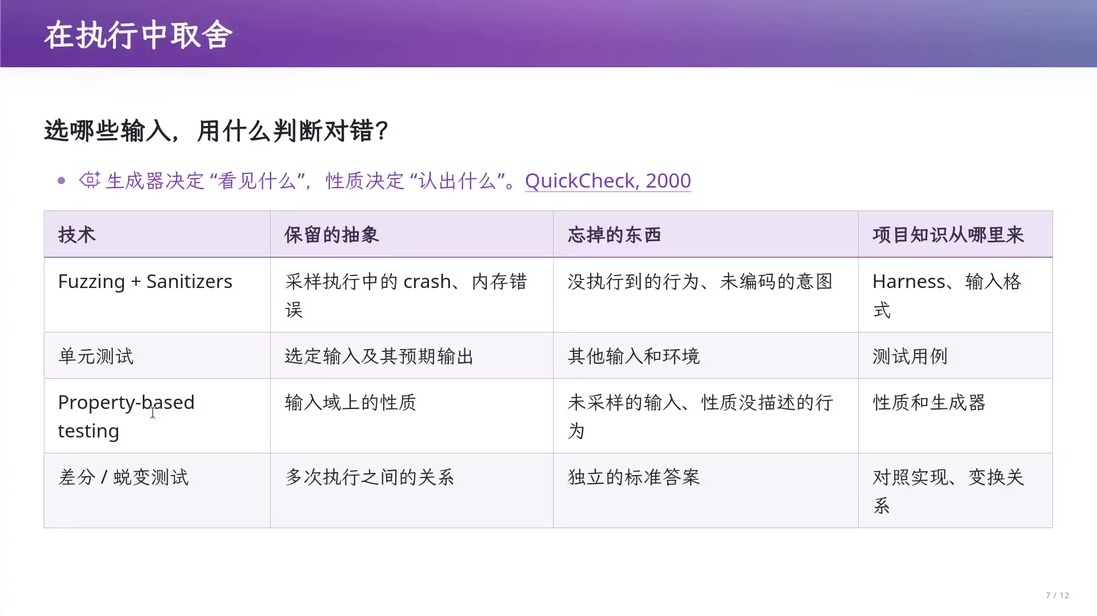
\includegraphics[width=0.88\textwidth]{figures/fig23_model_verification_tradeoff_table.jpg}
\caption{在模型中取舍（形式化验证篇）：“模型之外”没有消失，而是变成了需要单独核验的假设清单（如 seL4 的底层假设）\vtag}
\label{fig:fig23_model_verification_tradeoff_table}
\end{figure}
\srcnote{00:48:45--00:49:30}

因此，作为一名成熟的软件工程师或智能体架构师，当我们看到工具输出绿色的通过标志（\textbf{Pass $\checkmark$}）或红色的失败告警（\textbf{Fail $\times$}）时，绝不能盲目乐观或盲目恐慌，而必须清醒地追问（对应配图）：
\begin{center}
\textbf{看到绿色对勾（Pass），要问它究竟“买到了什么”？看到红色告警（Fail），要问它究竟“留下了什么证据”？}
\end{center}

\begin{figure}[H]
\centering
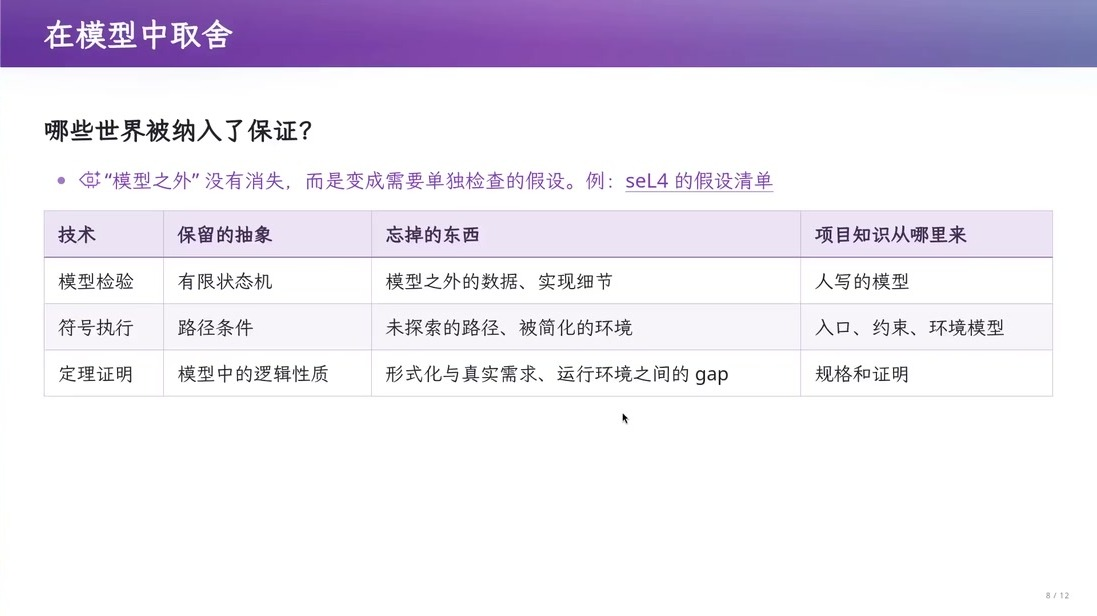
\includegraphics[width=0.88\textwidth]{figures/fig25_pass_vs_fail_static_table.jpg}
\caption{Pass 买到什么，Fail 留下什么（一）：类型系统、Linter 与抽象解释在通过与失败时的证据解读\vtag}
\label{fig:fig25_pass_vs_fail_static_table}
\end{figure}
\srcnote{00:56:15--00:56:38}

\begin{figure}[H]
\centering
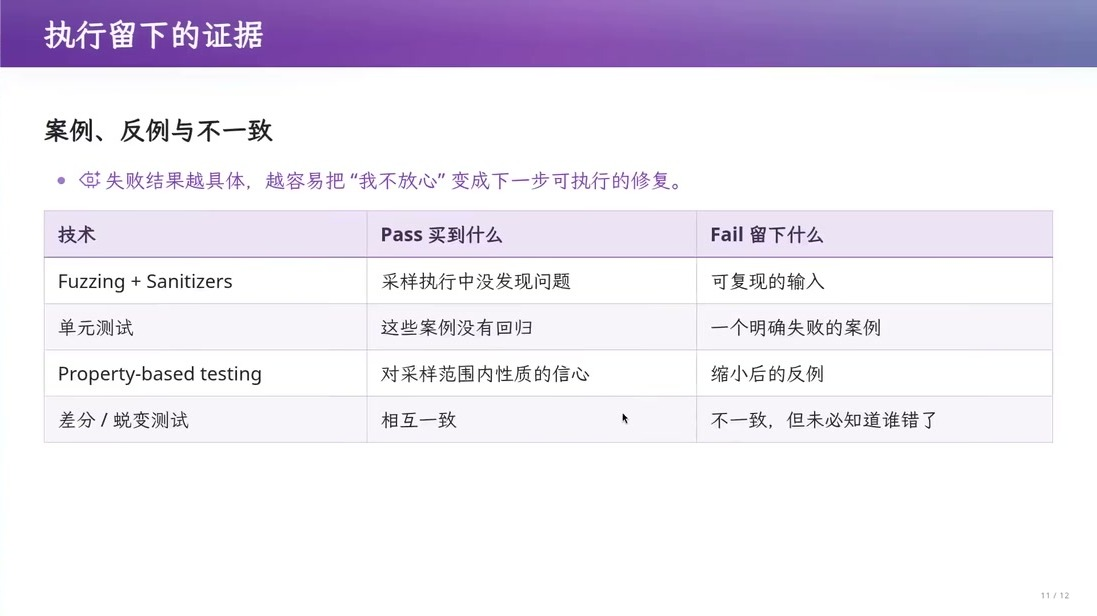
\includegraphics[width=0.88\textwidth]{figures/fig26_pass_vs_fail_verification_table.jpg}
\caption{验证留下的证据（二）：区分“找到真反例”与“没证出来”，才能决定下一步究竟是修程序，还是补规格、模型与引理\vtag}
\label{fig:fig26_pass_vs_fail_verification_table}
\end{figure}
\srcnote{00:56:40--00:57:02}

\begin{importantbox}{核心判读准则：不同工具在 Pass 与 Fail 时留下的证据形态}
综合两张证据判读表（对应配图），我们可以将所有软件分析工具的产出归纳为三类截然不同的后续行动指南：
\begin{enumerate}
    \item \textbf{留下可复现具体输入（Fuzzing / 单元测试 / 符号执行 Fail）}：拿到了铁证如山的触发输入 $x_{\text{crash}}$，下一步是直接挂载调试器复现并\textbf{修复程序代码}；
    \item \textbf{留下抽象状态或语法告警（Linter / 抽象解释 Fail）}：可能真的有风险，也可能是当前场景下不适用的误报（源于过近似 $\gamma(R^\#_{\text{abs}}) \supset R_{\text{conc}}$），下一步是\textbf{人工或交由 Agent 结合上下文甄别}；
    \item \textbf{留下未完成的证明目标（定理证明 Fail / Unknown）}：切忌一上来就乱改业务代码！未闭包的 Goal 往往只是因为归纳假设不够强或缺少辅助引理，下一步应当区分究竟是\textbf{修程序}，还是\textbf{补充规约、精化模型或添加引理}。
\end{enumerate}
\end{importantbox}

\subsection{工具带来的信心：为什么缩进混乱与残留文件让人“血压升高”？}

梳理完整个经典工具图谱后，主讲教师谈到了一个非常接地气的工程心理学现象（对应配图）：\textbf{为什么当老师或资深工程师打开一个学生的 Git 仓库，看到不一致的代码缩进、乱七八糟的运算符空格，以及一堆随手 `\texttt{git add .}` 塞进仓库的编译产物 `\texttt{a.out}` 和 macOS 隐藏文件 `\texttt{.DS\_Store}` 时，会瞬间“血压升高”？}

\begin{figure}[H]
\centering

\includegraphics[width=0.88\textwidth]{figures/fig24_confidence_and_formatting_signal.jpg}
\caption{工具带来的信心：每一种工具都在为黑盒软件提供可观察的反馈信号，而基础工程卫生则是判断维护者工程素养的强先验\vtag}
\label{fig:fig24_confidence_and_formatting_signal}
\end{figure}
\srcnote{00:49:35--00:54:55}

难道是因为缩进少两个空格会导致 CPU 算错指令吗？当然不是！这背后其实是一个极其严密的\textbf{贝叶斯后验信念更新（Bayesian Belief Update）}逻辑：
软件质量保障工具构成了一个从易到难的投入阶梯——最底层是只需肉眼扫一眼 `\texttt{git status}`、配一行 `\texttt{.gitignore}` 和自动格式化器（Formatter）就能做到的基础卫生；往上是 Linter、单元测试、Fuzzing；最顶层是模型检查与形式化证明。设代码库真正达到高质量标准的事件为 $H_{\text{good}}$，出现低级工程卫生混乱（如提交了 `\texttt{.DS\_Store}` 和 `\texttt{a.out}`）的观测事件为 $E_{\text{sloppy}}$。由于真正懂得并践行高阶质量保障的开发者极少会连最基础的 `\texttt{git diff}` 都不看（即似然比 $P(E_{\text{sloppy}} \mid H_{\text{good}}) \ll P(E_{\text{sloppy}} \mid \neg H_{\text{good}})$），根据贝叶斯公式：
\begin{equation}
\frac{P(H_{\text{good}} \mid E_{\text{sloppy}})}{P(\neg H_{\text{good}} \mid E_{\text{sloppy}})}
\;=\;
\underbrace{\frac{P(E_{\text{sloppy}} \mid H_{\text{good}})}{P(E_{\text{sloppy}} \mid \neg H_{\text{good}})}}_{\ll\, 1\text{（强负向证据）}}
\cdot
\frac{P(H_{\text{good}})}{P(\neg H_{\text{good}})}
\label{eq:bayesian_code_hygiene}
\end{equation}
一旦观察到 $E_{\text{sloppy}}$，审查者对“维护者用好了更高级的质量保障工具”的后验信心就会断崖式下跌！

更重要的是，在 AI 时代，人类几十年积累的这套软件分析工具链（Type Checker、Linter、Coverage、Sanitizer、Proof Assistant）共同构成了训练与驱动 Coding Agent 的\textbf{强化学习短程反馈飞轮（Short-horizon RL Feedback Flywheel）}：正是因为工具能够把黑盒代码转化为精确到行号的确定性报错信号，大模型才能在“生成 $\to$ 工具检查 $\to$ 定位修补”的闭环中高速自我博弈，最终在编码细节上超越人类手工极限。

% =========================================================================
% SECTION 6
% =========================================================================
\section{把程序作为概率分布的采样：软件自然性与承载两个世界的代码}

\subsection{打破“机械”假设：$\mathit{program} \sim P(\cdot \mid \mathit{intent}, \mathit{context}, \mathit{conventions})$}

在课程进入下半场（第 57 分钟）时，主讲教师提出了全讲最具颠覆性的理论转折：\textbf{为什么过去几十年所有的软件分析工具都无法真正替人类检查“代码是否符合真实需求”？因为整个传统软件分析领域都被困在了一个基本假设里——只把程序当成机械的形式语义对象，而忘了程序同时也是人类社会活动留下的概率采样样本！}（对应配图）

\begin{figure}[H]
\centering
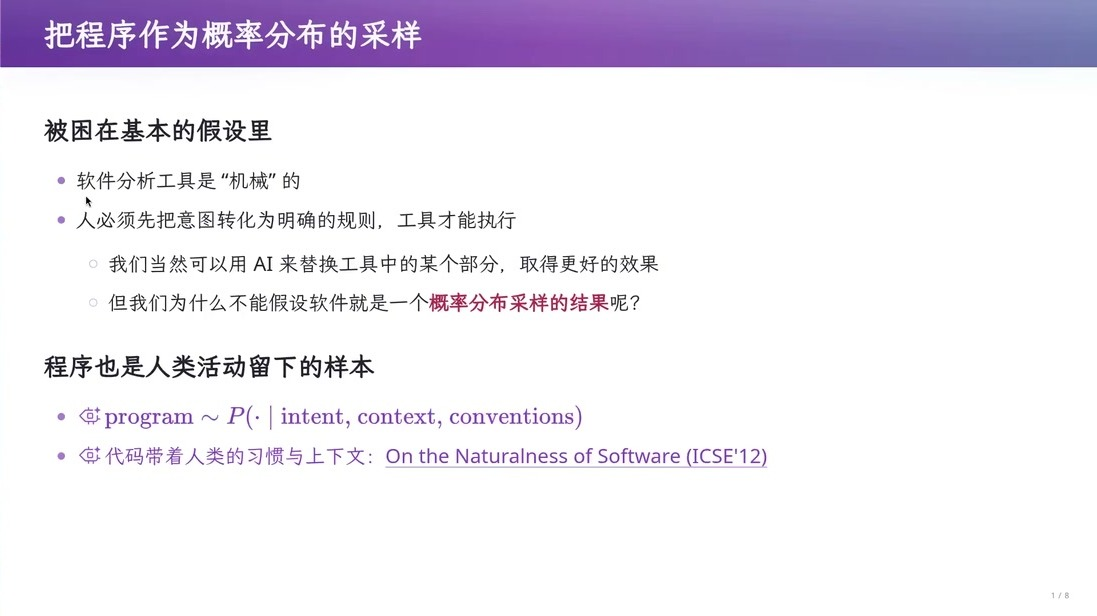
\includegraphics[width=0.88\textwidth]{figures/fig27_program_as_probability_sample.jpg}
\caption{把程序作为概率分布的采样：打破传统工具的机械假设，将代码视为条件概率分布 $\mathit{program} \sim P(\cdot \mid \mathit{intent}, \mathit{context}, \mathit{conventions})$ 的采样结果\vtag}
\label{fig:fig27_program_as_probability_sample}
\end{figure}
\srcnote{00:57:05--01:01:35}

当我们说“把程序看作概率分布的采样”时，绝不是说确定性的 CPU 下一秒会随机乱跳指令；而是指\textbf{代码的产生过程（Generation Process）}：当人类程序员（或受人类语料训练的 Agent）在特定的业务意图（$\mathit{intent}$）、项目上下文（$\mathit{context}$）与团队编程习惯（$\mathit{conventions}$）下编写代码时，最终落盘的那份源代码 $W = (w_1, w_2, \dots, w_T)$ 是从如下条件概率分布中采样出来的样本：
\begin{equation}
W \;\sim\; P\big(\mathit{program} \;\big|\; \mathit{intent},\; \mathit{context},\; \mathit{conventions}\big)
\label{eq:program_conditional_distribution}
\end{equation}

早在深度学习大模型爆发之前的 2012 年，Abram Hindle、Earl T. Barr、Zhendong Su、Mark Gabel 与 Premkumar Devanbu 就在软件工程顶会 ICSE 2012 上发表了极具前瞻性的奠基论文《On the Naturalness of Software》（对应配图下半部分）。他们指出：尽管编程语言在理论上允许写出任意古怪的语法组合，但真实人类写出的软件代码与人类自然语言（如英语文学作品）一样，具有极高的重复性与统计可预测性（即低信息熵 Low Entropy）。如果用 $N$-gram 马尔可夫语言模型（例如 $3$-gram，根据前两个 Token 预测下一个 Token）对代码 Token 序列建模：
\begin{equation}
P(w_1, w_2, \dots, w_T) \;\approx\; \prod_{i=1}^{T} P\big(w_i \;\big|\; w_{i-n+1}, \dots, w_{i-1}\big), \qquad
H(W) = -\frac{1}{T} \sum_{i=1}^{T} \log_2 P\big(w_i \;\big|\; w_{i-n+1}^{i-1}\big)
\label{eq:software_naturalness_ngram}
\end{equation}
就会发现真实代码库的交叉熵 $H(W)$ 甚至比自然语言还要低得多（通常仅需几比特）！这正是今天基于自回归 Next-Token Prediction 的大语言模型能够如此丝滑地生成、理解与修补代码的统计学根基。

\subsection{软件同时承载两个世界：从匿名函数 \texttt{f(x)} 到“芒果 TV”访问控制案例}

为什么公式 \eqref{eq:program_conditional_distribution} 如此重要？因为它揭示了一个被传统形式化分析彻底忽视的事实：\textbf{一份源代码同时承载着两个世界——对于 CPU 和传统静态分析器，它只是抽干了人类意义的符号与控制流；但对于人类和大语言模型，它的标识符命名（Identifiers）、常量与上下文注释里处处流淌着关于人类世界真实意图（Intent）的强信号！}

为了让大家一秒钟看懂“两个世界”的反差，主讲教师展示了一个令人忍俊不禁却又醍醐灌顶的课堂对比实验。首先看对应配图中被抹去所有具体名称的两段 Python 函数：

\begin{figure}[H]
\centering
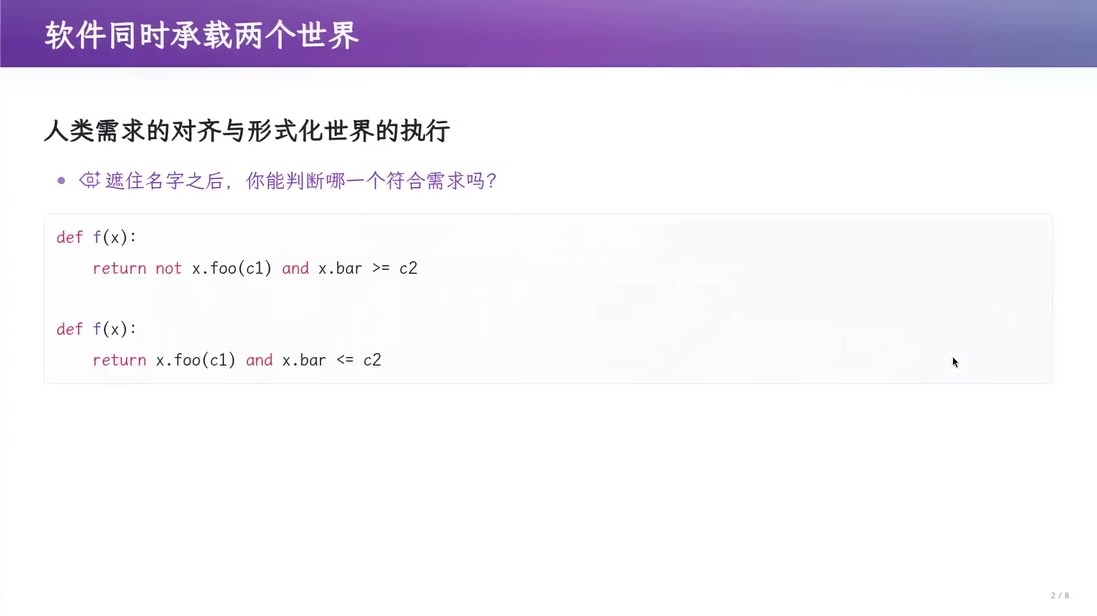
\includegraphics[width=0.88\textwidth]{figures/fig28_two_worlds_anonymized_code.jpg}
\caption{软件同时承载两个世界（遮住名字后）：面对两段只剩形式结构的匿名布尔函数 \texttt{f(x)}，任何分析器都无法判断哪一个符合需求\vtag}
\label{fig:fig28_two_worlds_anonymized_code}
\end{figure}
\srcnote{01:01:40--01:02:25}

\begin{lstlisting}[language=Python, caption={抹去标识符命名后的两段匿名函数（仅保留形式语义）}]
# 版本 A
def f(x):
    return not x.foo(c1) and x.bar >= c2

# 版本 B
def f(x):
    return x.foo(c1) and x.bar <= c2
\end{lstlisting}

请问：版本 A 和版本 B 哪一个写对了，哪一个有 Bug？
在传统静态分析器、类型检查器、Linter 乃至证明助手眼里，这两段代码的形式结构都是完全合法的（接收对象 `x`，调用方法 `foo` 取布尔值，并与属性 `bar` 的大小比较做逻辑与 `\texttt{and}`），条件个数也没有超标。脱离了人类世界，神仙也猜不出谁对谁错！

现在，让我们把标识符的名字和常量恢复回程序里（对应配图）：

\begin{figure}[H]
\centering
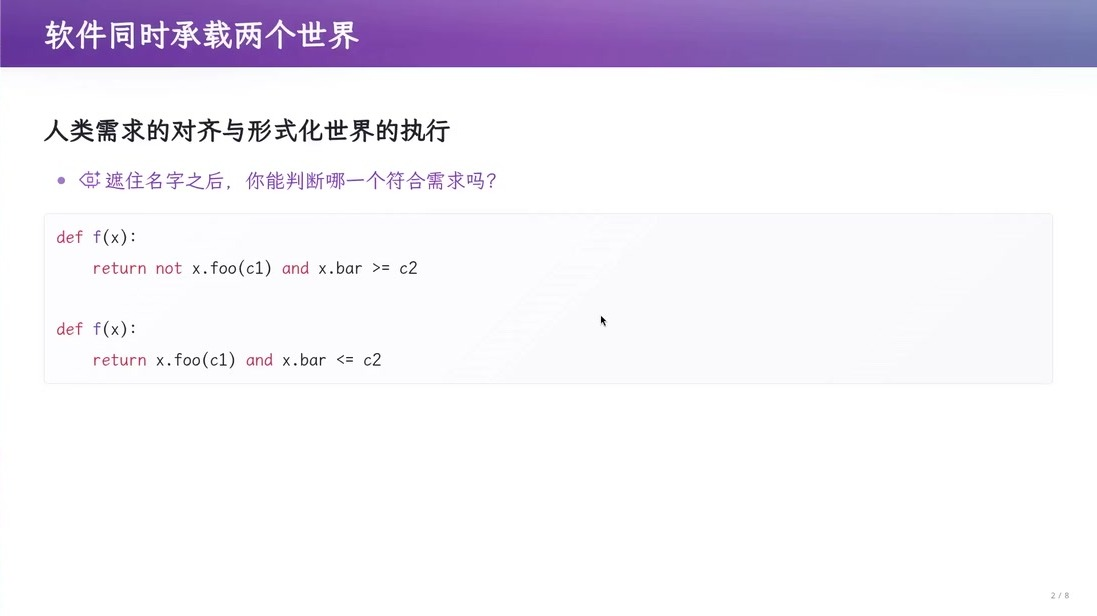
\includegraphics[width=0.88\textwidth]{figures/fig29_names_restored_mango_tv.jpg}
\caption{当名字回到程序里：恢复 `\texttt{can\_watch\_huang\_guo\_tv(visitor)}` 与 `\texttt{visitor.inside('China')}` 后，布尔运算瞬间接回了人类世界的常识与合规逻辑\vtag}
\label{fig:fig29_names_restored_mango_tv}
\end{figure}
\srcnote{01:02:30--01:03:15}

\begin{lstlisting}[language=Python, caption={恢复真实标识符与常量后的两段访问控制代码}]
# 版本 A：允许中国境外、且年满 18 周岁的成年访客观看
def can_watch_huang_guo_tv(visitor):
    return not visitor.inside('China') and visitor.age >= 18

# 版本 B：仅允许中国境内、且年龄不超过 18 周岁的未成年访客观看
def can_watch_huang_guo_tv(visitor):
    return visitor.inside('China') and visitor.age <= 18
\end{lstlisting}

就在名字恢复的一刹那，全场会心一笑——原本冰冷的布尔表达式瞬间接通了人类世界的常识背景！即便我们手头还没有拿到该视频平台的正式产品需求文档，任何一个具备人类常识的工程师（或大语言模型）看到这两个版本时，也立刻知道应该去质疑和核对什么：为什么一个叫 `\texttt{huang\_guo\_tv}` 的平台要限制境内访问但要求年满 $18$ 岁（版本 A），或者反过来只允许境内 $18$ 岁以下未成年人观看（版本 B，难不成是少儿频道）？

\begin{knowledgebox}{核心洞见：标识符命名是连接形式化执行世界与人类意图世界的虫洞}
在传统编译原理中，变量名 `\texttt{visitor}` 与 `\texttt{x}` 在词法分析之后就会被替换为符号表编号，二者毫无区别；但在公式 \eqref{eq:program_conditional_distribution} 的概率生成视角下，标识符命名携带了极高密度的互信息 $I(\mathit{Names};\, \mathit{Intent})$。当大语言模型读到函数名与字段名时，它便能从条件分布 $P(\mathit{Intent} \mid \mathit{Code})$ 中反向推断出代码原本试图解决的人类问题，从而第一次让软件分析工具具备了“质疑业务语义是否写反”的能力！
\end{knowledgebox}

% =========================================================================
% SECTION 7
% =========================================================================
\section{非形式化验证（Informal Verification）与“Mechanism Is King”}

\subsection{为什么 AI 时代仍需要确定性软件？——9 个数量级的能效鸿沟与 Informal Verification}

既然大语言模型如此擅长理解人类意图，甚至今天已经有研究尝试用生成式世界模型直接实时渲染游戏画面，那么有人难免会问：\textbf{未来我们还需要编写确定性的软件代码（Implementation）吗？为什么不让大模型直接接管一切计算？}

主讲教师从物理与计算机体系结构的第一性原理给出了斩钉截铁的回答：\textbf{因为 CPU 执行确定性指令的能效比（Energy Efficiency），比大语言模型做神经网络推理高出整整约 9 个数量级（$10^9$ 倍）！}
\begin{equation}
\frac{E_{\text{LLM Inference}}(\text{per logical operation})}{E_{\text{CPU Deterministic Instruction}}(\text{per ALU/DB op})} \;\approx\; 10^9 \quad (\text{约九个数量级的能耗与成本差距})
\label{eq:cpu_vs_llm_energy_gap}
\end{equation}
在现代硅基芯片上，一次 64 位整数加法或一次确定性的数据库持久化写入仅消耗皮焦耳（$\mathrm{pJ}$）乃至纳焦耳（$\mathrm{nJ}$）量级的能量，且一旦程序逻辑正确，执行一万亿次也绝不会因为“今天心情不好”或“提示词多了一个空格”而产生随机幻觉；相比之下，让百亿参数大模型通过自回归矩阵乘法去完成同样的状态维护，消耗的电力与金钱是地球资源根本无法承受的。因此，\textbf{凡是能够固化为确定性规则的计算，最终依然必须沉淀为 CPU 上运行的软件（Implementation）}！

既然软件实现 $C$ 依然不可或缺，那么在 AI 时代，软件分析工具的终极使命就变得前所未有地清晰——主讲教师将其正式命名为\textbf{非形式化验证（Informal Verification）}（对应配图）：

\begin{figure}[H]
\centering
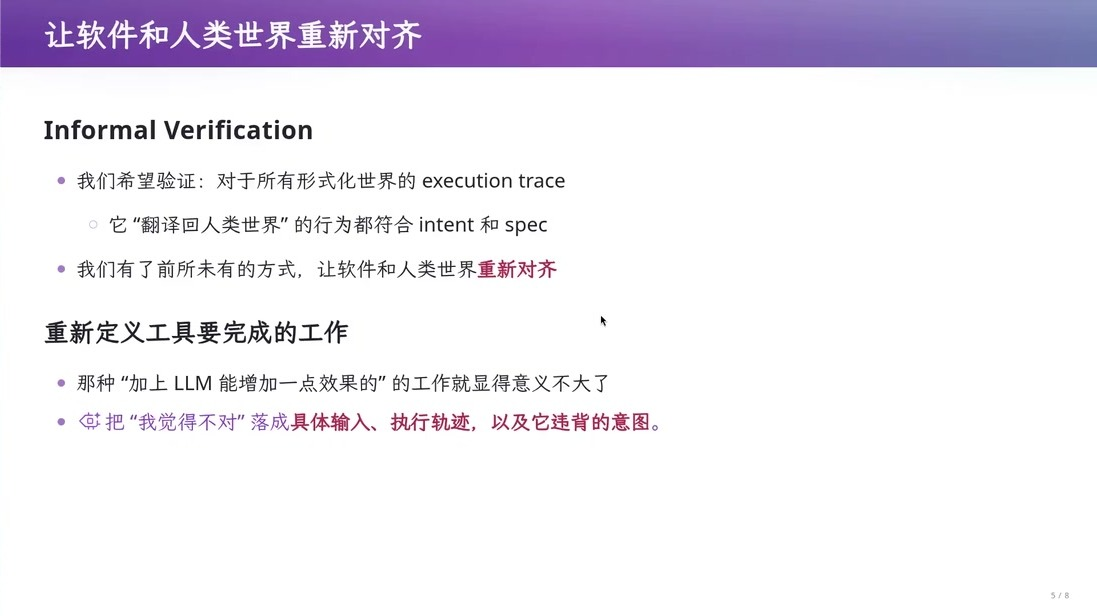
\includegraphics[width=0.88\textwidth]{figures/fig30_informal_verification_alignment.jpg}
\caption{让软件和人类世界重新对齐——Informal Verification：检查形式化世界中的每条执行轨迹（Execution Trace）翻译回人类世界后是否符合 Intent 与 Spec\vtag}
\label{fig:fig30_informal_verification_alignment}
\end{figure}
\srcnote{01:03:20--01:07:50}

\begin{figure}[H]
\centering
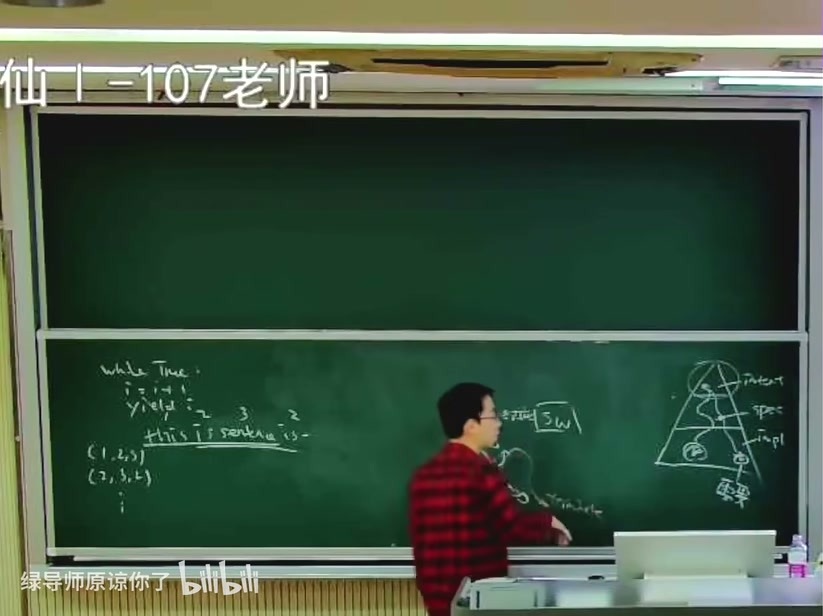
\includegraphics[width=0.72\textwidth]{figures/fig31_board_formal_informal_bridge.jpg}
\caption{黑板板书：对状态机中的任意执行轨迹 $\forall \mathit{trace}$，通过大模型将其语义投射回人类世界，核验 $\mathrm{Align}(\mathit{trace}, \mathit{Intent} \land \mathit{Spec})$\vtag}
\label{fig:fig31_board_formal_informal_bridge}
\end{figure}
\srcnote{01:05:30--01:07:45}

如对应配图与黑板板书所示，过去的形式化验证只关心程序在形式语义内部是否满足机械属性（如 `\texttt{no null-pointer dereference}`、`\texttt{no integer overflow}`）；而 **Informal Verification** 的目标是：对于软件状态机 $\mathcal{M}_C$ 产生的任意执行轨迹 $\tau \in \mathrm{Traces}(\mathcal{M}_C)$，利用语义翻译映射 $\mathcal{T}_{\text{human}}$ 将其还原为人类世界的业务行为描述，并检验它是否与人类的真实意图（$\mathit{Intent}$）及非形式化规约（$\mathit{Spec}$）对齐：
\begin{equation}
\mathsf{InformalVerify}(\mathcal{M}_C) \triangleq
\forall \tau \in \mathrm{Traces}(\mathcal{M}_C):\;
\mathrm{Judge}\big(\mathcal{T}_{\text{human}}(\tau), \mathit{Intent}, \mathit{Spec}\big) = \mathsf{Aligned}
\label{eq:informal_verification_def}
\end{equation}
更有价值的是，Informal Verification 绝不是让大模型笼统地看一眼代码说句“我觉得年龄条件写反了”就完事，而是\textbf{要求工具把大模型的怀疑落地为具体的测试输入 $x_{\text{suspect}}$、真实的执行轨迹 $\tau(x_{\text{suspect}})$ 以及需要向人类澄清的意图问题}！

\subsection{Heuristics Is Dead, Policy Is Heuristics, LLM Is Policy, Mechanism Is King!}

当大模型接管了公式 \eqref{eq:informal_verification_def} 中的非形式化语义评判后，整个软件分析工具的设计哲学将发生怎样的重构？主讲教师改编了图灵奖得主 Jim Gray 在 \textbf{06年}（2006 年 12 月）关于存储层次结构演进的著名论断，提出了本讲最核心的架构口号（对应配图）：

\begin{figure}[H]
\centering
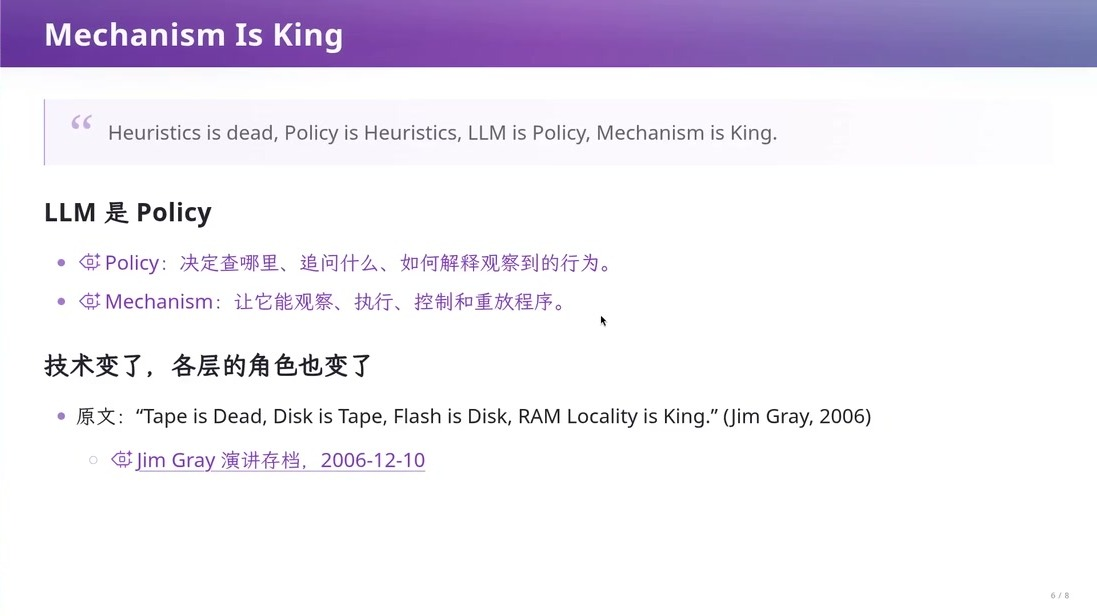
\includegraphics[width=0.88\textwidth]{figures/fig32_mechanism_is_king_jim_gray.jpg}
\caption{Mechanism Is King：致敬 Jim Gray（06年）名言——“Heuristics is dead, Policy is Heuristics, LLM is Policy, Mechanism is King”\vtag}
\label{fig:fig32_mechanism_is_king_jim_gray}
\end{figure}
\srcnote{01:07:55--01:10:45}

在 \textbf{06年}闪存（Flash SSD）刚刚兴起时，Jim Gray 曾预言：
\begin{quote}
\textit{``Tape is Dead, Disk is Tape, Flash is Disk, RAM Locality is King.''}\\
（磁带已死，磁盘沦为昔日的顺序磁带，闪存取代昔日的随机磁盘，而内存局部性为王——这一论断甚至精准预言了今天 GPU 高带宽显存 HBM 局部性决定大模型生死的时代！）
\end{quote}
\begin{importantbox}{范式宣言：Heuristics is dead, Policy is Heuristics, LLM is Policy, Mechanism is King!}
在传统软件分析中，由于工具缺乏理解人类业务常识的能力，研究者被迫设计各种僵化的数字启发式（如强制要求单元测试覆盖率达到 80\% 或 90\%，Fuzzing 达到 95\% 或 99\%）来近似软件质量。而在大模型时代，决定“测哪里、查什么、如何理解反例”的策略层（Policy）应当全面移交给具备人类世界先验的 LLM；软件工程工具的核心价值则回归到提供可靠执行、低开销全迹观测、状态快照重放与结构化视图投影的底层机制（Mechanism）。
\end{importantbox}

对照这一存储层级的角色位移，主讲教师为 AI 时代的软件分析工具写下了完全同构的四句箴言：
\begin{equation}
\textbf{Heuristics is dead,\quad Policy is Heuristics,\quad LLM is Policy,\quad Mechanism is King.}
\label{eq:mechanism_is_king_slogan}
\end{equation}

如何深刻理解公式 \eqref{eq:mechanism_is_king_slogan} 的每一层含义？
\begin{enumerate}
    \item \textbf{为什么说“Heuristics is dead（传统手写启发式已死）”？}
    在没有大模型之前，因为工具是人写的死程序，人类无法把复杂的业务重要性写进规则，只能发明各种粗糙的数字启发式（Heuristics）来凑合。最典型的例子就是前面提到的代码覆盖率阈值：为什么团队规定单元测试覆盖率到底是 80\% 还是 90\%，加上 Fuzzing 后是不是达到了 95\% 或者 99\%？请问为什么是 \textbf{95\%} 或 \textbf{99\%} 就够了？你完全可能刷满了 \textbf{99\%} 的边缘 getter/setter 代码，而偏偏漏掉了那 $1\%$ 最致命的核心资金结算分支！过去那些为了把某个静态分析器的启发式排序指标从 \textbf{80\%} 刷到 \textbf{90\%} 的套路式论文，在今天已经失去了根本意义。
    \item \textbf{为什么说“Policy is Heuristics, LLM is Policy（大模型就是新的策略层）”？}
    在操作系统与系统设计中，\textbf{策略（Policy，决定“查哪里、追问什么、如何解释观测结果”）}与\textbf{机制（Mechanism，提供“如何可靠地观测、执行、控制和重放程序”）}应当严格分离。过去写死在工具里的启发式策略，如今完全应该交给具备人类世界常识的 \textbf{LLM} 来动态决策！
    \item \textbf{为什么说“Mechanism is King（底层机制为王）”？}
    当 LLM 接管了策略层之后，软件工程工具研究者真正应该发力的核心战场，就是打造极致强大、零幻觉、低开销的\textbf{底层机制（Mechanism）}——例如：如何让 Agent 以极低开销观测任意执行轨迹？如何瞬间冻结、分支克隆并确定性重放一个分布式系统状态？如何将复杂的内存指针图精准投射为模型与人类可读的视图？没有坚如磐石的 Mechanism，再聪明的 LLM Policy 也只是瞎子摸象！
\end{enumerate}

% =========================================================================
% SECTION 8
% =========================================================================
\section{从日志挖掘、图形调试器到“No Doc”哲学：构建有“人感”的软件视图}

为了具体展示什么样的机制（Mechanism）能够帮助人类与大模型实现非形式化验证（Informal Verification），主讲教师深入剖析了两个跨越十余年的经典系统工具案例：一个是 **SOSP 2009 的控制台日志异常挖掘**，另一个是 **SIGPLAN Notices 1996 的 GNU DDD 图形化调试器**。

\subsection{案例一：从控制台日志学习正常运行模式（SOSP'09）与非形式化语义恢复}

很多严重的线上系统故障既不会触发段错误（Crash），也不会违背局部断言，但人类老手一看运行轨迹就知道“不对劲”——比如在玩 3D 射击游戏时，角色坐标平时都在地图平面有界范围内移动，突然有一帧角色“穿模”掉进了地底深渊（$z$ 轴坐标向 $-\infty$ 狂跌）。这种“很难事前写成死规则，但偏离正常历史分布”的异常，该如何自动捕捉？

早在 \textbf{2009年}（SOSP'09），加州大学伯克利分校的 Wei Xu、Ling Huang、Armando Fox、David Patterson 与 Michael I. Jordan 就发表了一篇开创性论文《Detecting Large-Scale System Problems by Mining Console Logs》（对应配图）：

\begin{figure}[H]
\centering
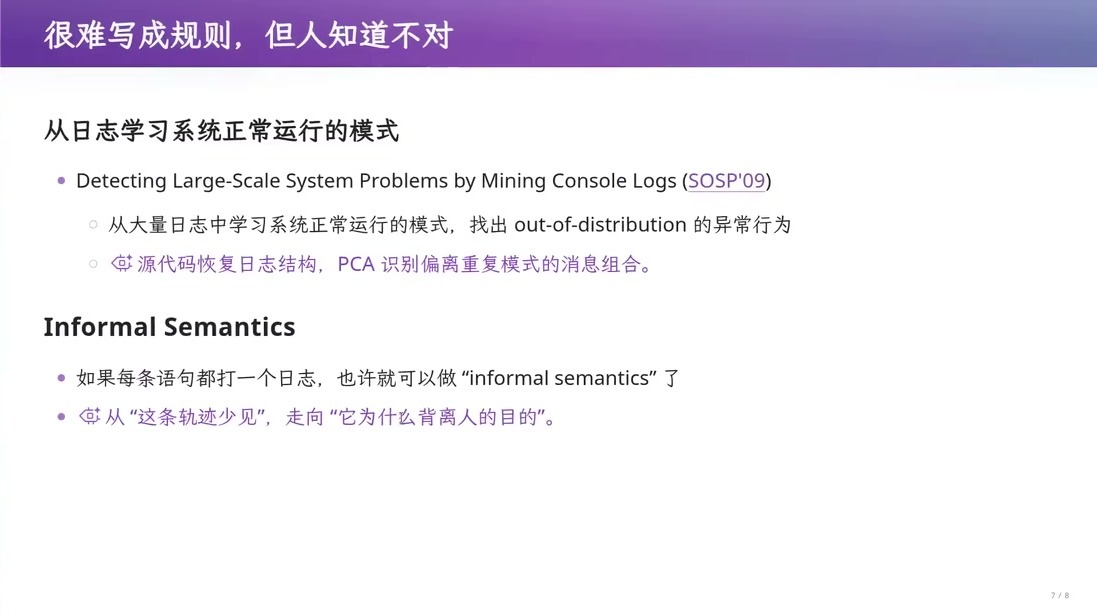
\includegraphics[width=0.88\textwidth]{figures/fig33_log_mining_sosp09_informal_semantics.jpg}
\caption{很难写成规则，但人知道不对：Xu 等人（SOSP'09）从海量控制台日志中用 PCA 识别异常行为，以及通过全语句日志恢复 Informal Semantics 的构想\vtag}
\label{fig:fig33_log_mining_sosp09_informal_semantics}
\end{figure}
\srcnote{01:10:50--01:11:35}

\begin{figure}[H]
\centering
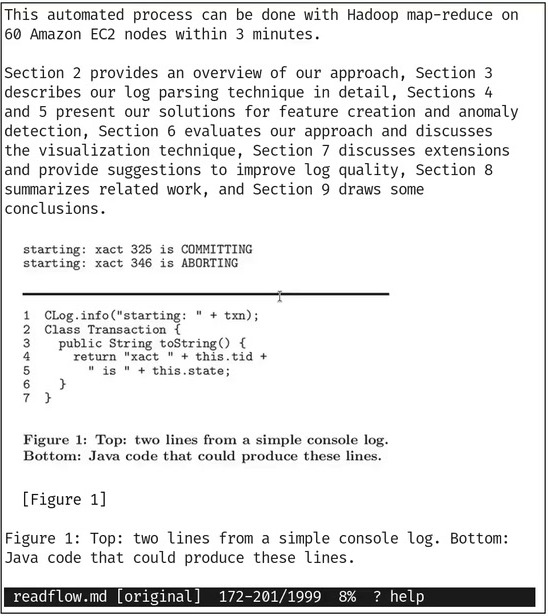
\includegraphics[width=0.80\textwidth]{figures/fig34_sosp09_xu_console_logs_paper.jpg}
\caption{文献精读：在 \textbf{2009年} SOSP 论文中，作者利用源码 AST 提取 `\texttt{clog.info("starting: " + txn)}` 日志模板与对象标识符，在 60 台 EC2 节点上 3 分钟完成分析\vtag}
\label{fig:fig34_sosp09_xu_console_logs_paper}
\end{figure}
\srcnote{01:11:40--01:16:35}

如对应配图所示，这篇 \textbf{2009年}的论文展示了一套极具巧思的机制设计：
\begin{enumerate}
    \item \textbf{结合源代码 AST 恢复结构化日志模板}：自由文本日志（如 `\texttt{starting: each 325 is COMMITTING}`）很难直接做统计。作者扫描程序的 Java 源代码（如 `\texttt{clog.info("starting: " + txn)}`），自动分离出静态的**日志消息模板（Message Type）**与动态的**业务对象/事务标识符（State Ratio / Variable IDs）**；
    \item \textbf{特征矩阵构造与主成分分析（PCA）异常检测}：按事务 ID 将千万条日志分组，把每个事务生命周期内各日志模板出现的频次编码为一个特征向量 $\vec{y} \in \mathbb{R}^m$。假设正常业务流程总是依次打印模板 $A \to B \to C$，而某次异常执行却打印了 $C \to B \to A$。通过主成分分析（PCA）将向量 $\vec{y}$ 投影到正常主子空间，并计算其在残差子空间（Residual Subspace）上的投影长度（即平方预测误差 SPE / $Q$-statistic）：
    \begin{equation}
    \mathrm{SPE}(\vec{y}) = \big\| (I - P_k P_k^\top)\, \vec{y} \big\|_2^2 > \delta_{\alpha}
    \;\Longrightarrow\;
    \text{判定为分布外异常轨迹（Anomaly）}
    \label{eq:pca_log_anomaly_spe}
    \end{equation}
\end{enumerate}

\begin{figure}[H]
\centering
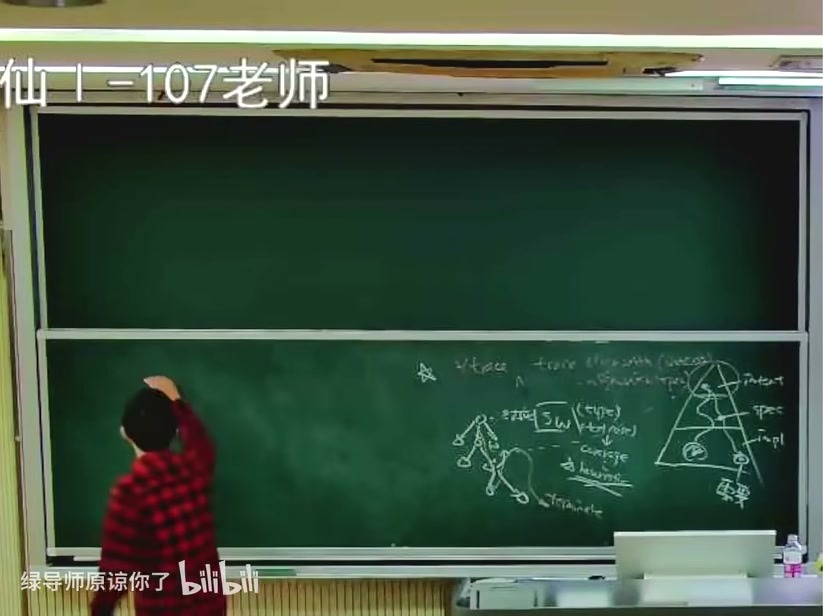
\includegraphics[width=0.72\textwidth]{figures/fig35_board_execution_log_trajectory.jpg}
\caption{黑板板书：左侧展示每条语句附带自然语言意图日志的插桩，右侧展示物理坐标轨迹中穿模跌落（Outlier）的异常检测\vtag}
\label{fig:fig35_board_execution_log_trajectory}
\end{figure}
\srcnote{01:14:30--01:17:50}

站在今天大模型的视角回看 \textbf{2009年}的这项工作，主讲教师提出了一个更大胆的演进设想（对应配图）：以前程序员写下一行函数调用时，脑子里明明清楚这行代码在业务上要干什么，但落成代码后这些上下文信息就丢失了（以至于静态分析界花了几十年研究指针分析与 Call Graph 恢复）。如果我们在生成式软件工程中建立一种新机制——\textbf{在编译或运行插桩时，让每一条基本块或关键语句都自动附带一段面向人类意图的结构化微日志（Micro-log of Intent）}，那么程序运行一次所产生的日志流，就不再是干瘪的十六进制地址，而是一份可以直接喂给大模型做 Informal Verification 的\textbf{非形式化语义轨迹（Informal Semantics Trace）}！工具不仅能指出“这条轨迹罕见”，还能直接回答“为什么这次用户请求违背了原本的业务目的”。

\subsection{案例二：有“人感”的软件视图（GNU DDD 图形调试器）与“No Doc”哲学}

除了日志轨迹之外，软件分析工具的另一个重要方向是**把机器内部晦涩的状态投射为人类（及多模态模型）一眼就能看懂的“有人感”的视图**（对应配图）。

\begin{figure}[H]
\centering
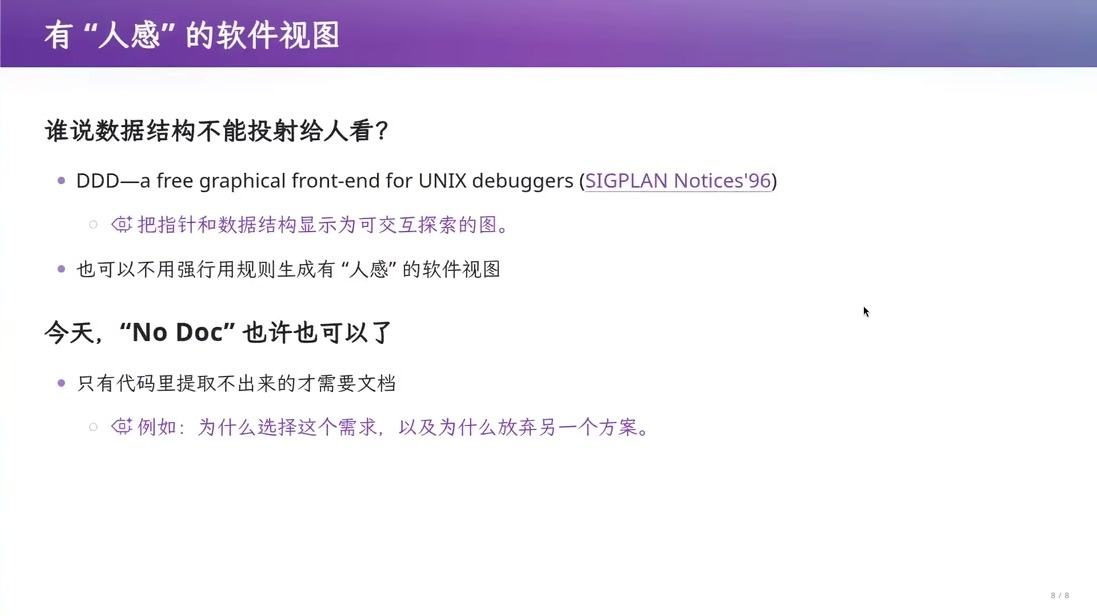
\includegraphics[width=0.88\textwidth]{figures/fig36_human_sense_views_ddd_nodoc.jpg}
\caption{有“人感”的软件视图：从 Andreas Zeller 的 DDD 图形调试器（SIGPLAN Notices'96）到 AI 时代的“No Doc”文档哲学\vtag}
\label{fig:fig36_human_sense_views_ddd_nodoc}
\end{figure}
\srcnote{01:17:55--01:18:18}

凡是在数据结构课上手写过 AVL 树或红黑树旋转的同学，都有过对着段错误或乱序输出抓狂的经历：当树里的某个指针指错时，用 `\texttt{printf}` 打印出来的满屏十六进制地址只会让人越看越心烦气躁。而在 1996 年，软件调试领域的泰斗 Andreas Zeller（与 Dorothea Lütkehaus 合作）发表了他的成名作——\textbf{GNU DDD（Data Display Debugger）}（对应配图）：

\begin{figure}[H]
\centering
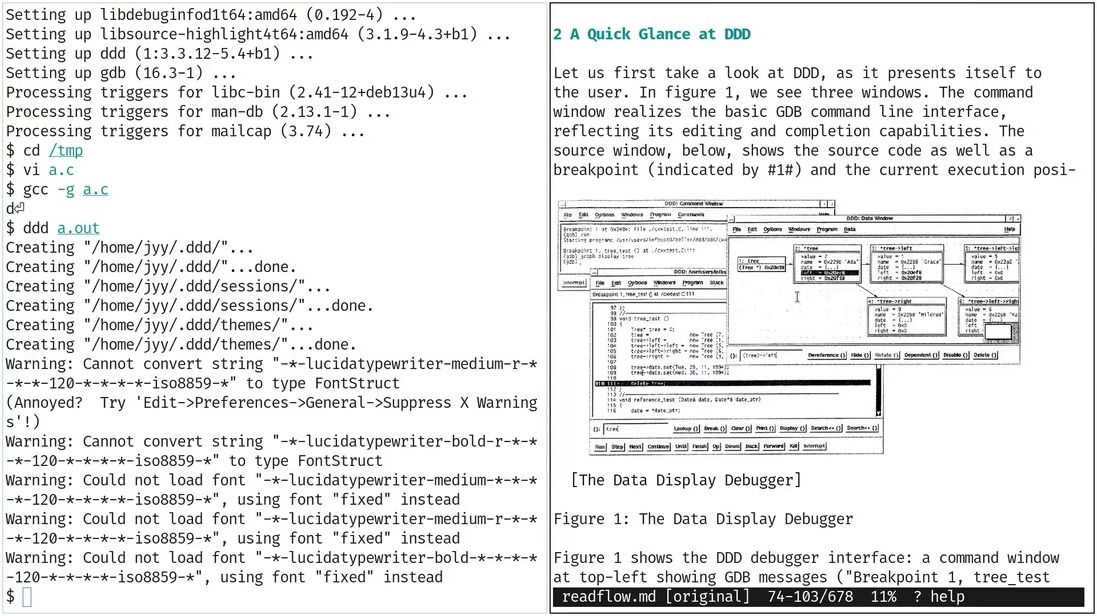
\includegraphics[width=0.88\textwidth]{figures/fig37_ddd_live_demo_and_paper.jpg}
\caption{终端编译与文献同屏演示：左侧现场安装并启动 DDD 调试器，右侧展示 Zeller（1996）论文中将 C 指针链表/树结构实时渲染为可交互图形框图\vtag}
\label{fig:fig37_ddd_live_demo_and_paper}
\end{figure}
\srcnote{01:18:20--01:20:45}

\begin{figure}[H]
\centering
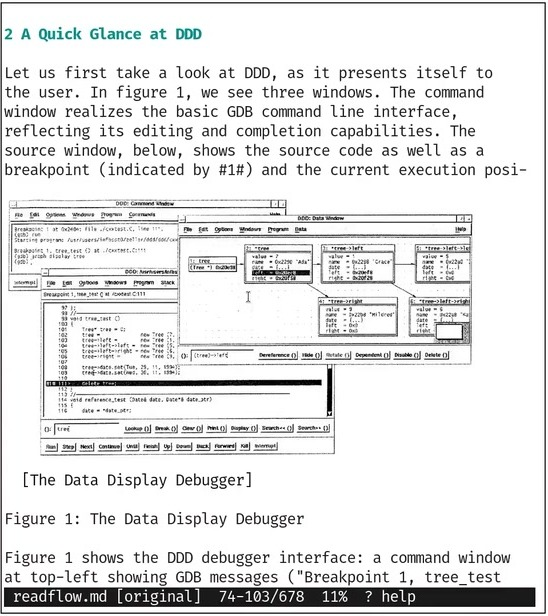
\includegraphics[width=0.80\textwidth]{figures/fig38_ddd_paper_architecture_diagram.jpg}
\caption{文献精读：DDD 论文展示前端 GUI 如何通过异步命令队列驱动底层 GDB，将内存状态解析并投射为人类可读的视觉图形\vtag}
\label{fig:fig38_ddd_paper_architecture_diagram}
\end{figure}
\srcnote{01:20:50--01:21:12}

如对应配图所示，DDD 本质上是架在传统命令行调试器（GDB / DBX）之上的一个图形化视图投影层：它通过异步命令队列向底层 GDB 查询结构体字段与指针指向，并将链表、二叉树或图直接绘制在画布上，让原本隐藏在内存地址背后的结构错误无所遁形。在今天，我们完全可以把 DDD 的思想升级为**由大模型按需驱动的动态视图合成**：不再局限于固定规则的指针画图，而是将海量内核或分布式状态压缩、过滤并投射为针对当前调试任务的紧凑语义视图。

沿着“按需从代码合成视图”的思路继续推演，主讲教师提出了极具冲击力的 \textbf{“No Doc”工作模式}（对应配图下半部分）：
\begin{practicebox}{AI 时代的“No Doc”工程哲学：什么文档该彻底消灭，什么文档必须保留？}
在传统软件工程中，人们总强调“要多写设计文档与代码说明文档”；但在 Agent 时代，静态检入 Git 仓库的代码描述文档极易在代码修改后沦为过期的毒药（误导下一轮 Agent 会话）。因此，“No Doc”哲学主张对文档做严格的二分切割：
\begin{enumerate}
    \item \textbf{凡是能从代码本身推导提取出的结构与行为描述（What \& How）——绝不手写、绝不检入 Git 仓库！}应当将其视为类似编译产物 `\texttt{a.out}` 的派生视图，通过专门的 \texttt{Skill} 在 CI/CD 或阅读时按需动态生成（为新手生成入门导览视图、为架构师生成模块依赖视图、为 Informal Verification 生成语句级意图注释）；
    \item \textbf{唯有从代码里绝对提取不出来的“决策理由与被否决方案”（Why \& Why Not）——才是真正必须长期维护的核心文档！}例如：“为什么我们选择了当前这个看似拧巴的需求边界？”“为什么我们明确放弃了另外三种看似更简单的架构方案？”“哪条奇怪的限制来自外部硬件或合规铁律？”因为大模型可以读懂代码结果，却永远无法仅凭结果反推出所有历史权衡的初衷。
\end{enumerate}
\end{practicebox}

% =========================================================================
% SECTION 9
% =========================================================================
\section{软件工程工具的未来：三圆交集、架构泥潭与从第一性原理重构软件}

\subsection{2024 年的三圆维恩图：语法正确、阅读自然与语义正确}

在本讲的最后部分，主讲教师展示了一张他在 \textbf{2024年}制作幻灯片时绘制的“软件生成三大目标维恩图”（对应配图），以此审视生成式软件工程走过的路与未来的终局：

\begin{figure}[H]
\centering
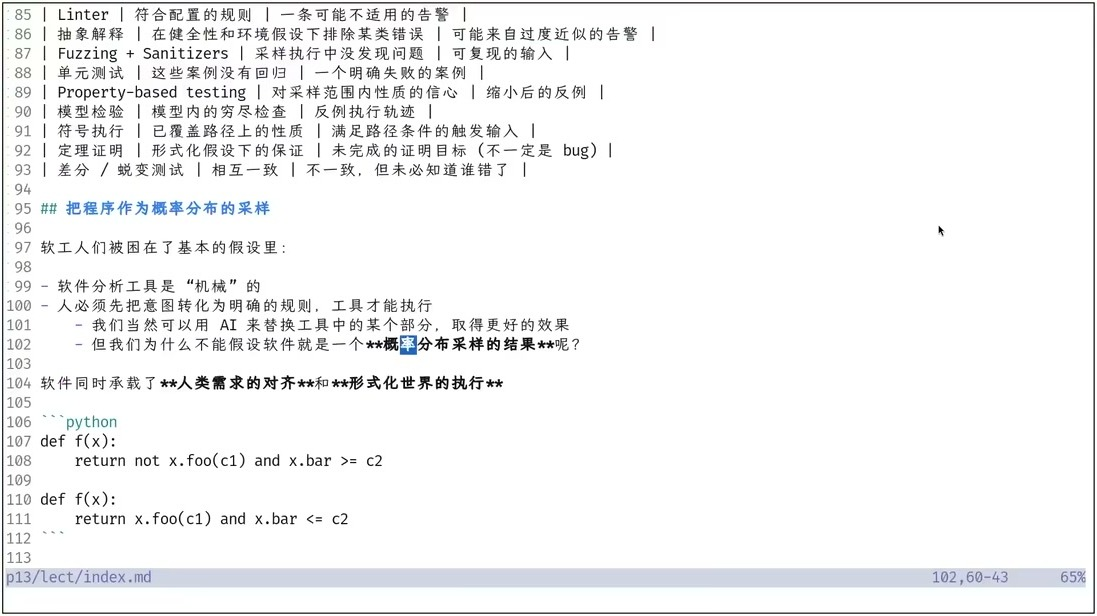
\includegraphics[width=0.88\textwidth]{figures/fig39_future_three_circles_venn.jpg}
\caption{软件工程工具的未来（源自 \textbf{2024年}讲义图）：语法正确（符号主义搜索）、阅读自然（大语言模型）与语义正确（Open Problem）的三圆交集\vtag}
\label{fig:fig39_future_three_circles_venn}
\end{figure}
\srcnote{01:25:50--01:27:00}

如对应配图所示，一份真正理想的软件制品 $P^*$ 必须同时落入三个集合的交集：
\begin{equation}
P^* \;\in\; \mathcal{C}_{\text{syntax}}\text{（语法正确）} \;\cap\; \mathcal{C}_{\text{natural}}\text{（阅读自然）} \;\cap\; \mathcal{C}_{\text{semantic}}(\mathit{Intent}, \mathit{Spec})\text{（语义正确）}
\label{eq:three_circles_intersection}
\end{equation}
\begin{itemize}
    \item \textbf{语法正确（$\mathcal{C}_{\text{syntax}}$）}：这是符号主义时代（编译器、语法制导程序合成 Syntax-Guided Synthesis）的主场，保证程序能通过词法、语法与静态类型检查；
    \item \textbf{阅读自然（$\mathcal{C}_{\text{natural}}$）}：这是深度学习、大语言模型与 Beam Search 的拿手好戏，保证生成的代码符合人类命名与排版习惯，读起来像模像样；
    \item \textbf{语义正确（$\mathcal{C}_{\text{semantic}}$）}：在 \textbf{2024年}前后，如何让生成的代码真正符合人类的需求与规格（而非 SWE-bench 早期那样漏洞百出），曾是一个巨大的 \textbf{Open Problem}。
\end{itemize}

\subsection{Open Problem 真的被解决了吗？——警惕试错修补带来的“架构泥潭”}

到了 2026 年的今天，随着 Coding Agent 学会了熟练调用我们前面介绍的整套软件工程工具（编译器、Linter、单元测试、Fuzzing、截图对比），公式 \eqref{eq:three_circles_intersection} 中的“语义正确”看似在很大程度上已经被攻克了。它的工作机制可以概括为一条**受工具反馈引导的迭代采样轨迹**：
\begin{equation}
P_0 \sim P(\cdot \mid \mathit{Prompt})
\xrightarrow{f(P_0)}
P_1
\xrightarrow{f(P_1)}
\cdots
\xrightarrow{\text{Pass}}
P_k \in \mathcal{C}_{\text{syntax}} \cap \mathcal{C}_{\text{natural}} \cap \mathcal{C}_{\text{semantic}}
\label{eq:agent_trial_and_error_trajectory}
\end{equation}
即 Agent 先在 $\mathcal{C}_{\text{syntax}} \cap \mathcal{C}_{\text{natural}}$ 中盲猜一个初始采样点 $P_0$，然后跑测试、看报错、打补丁，一路磕磕绊绊修到所有工具都亮起绿灯的 $P_k$。

然而，主讲教师在最后一张幻灯片上敲响了振聋发聩的警钟：\textbf{这种靠“局部试错（Trial and Error）$+$ 工具反馈修补”的模式，真的从根本上（Fundamentally）解决软件工程的构建难题了吗？答案是：只解决了一定程度，而且极其低效、极易陷入无法维护的架构泥潭！}（对应配图）

\begin{figure}[H]
\centering
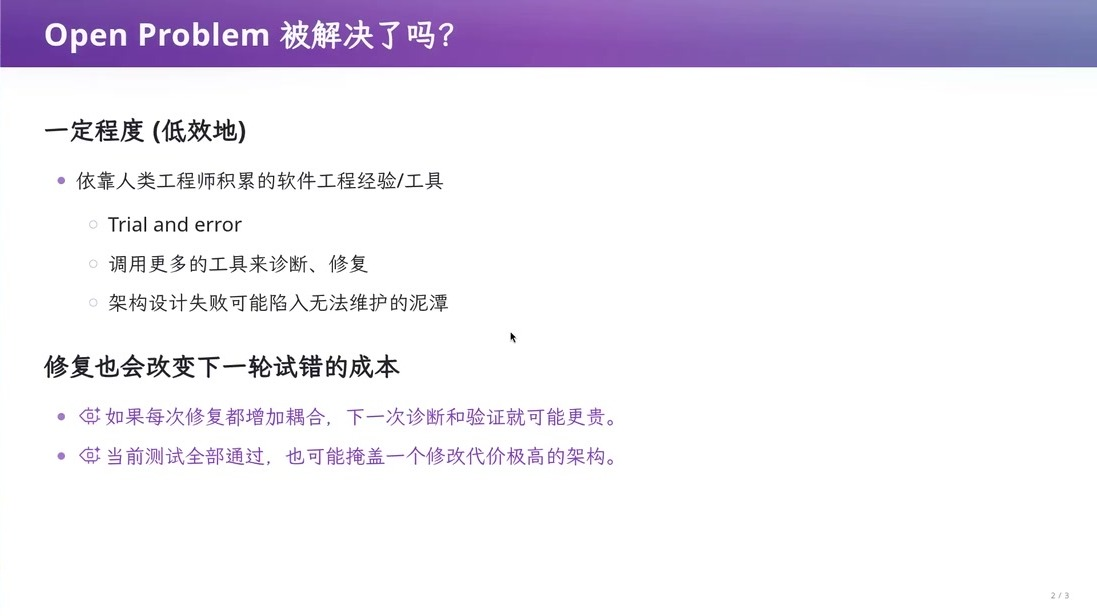
\includegraphics[width=0.88\textwidth]{figures/fig40_open_problem_architecture_mud.jpg}
\caption{Open Problem 被解决了吗：单次测试通过可能掩盖修改代价高昂的烂架构，每次试错修补若增加耦合，最终将陷入无法维护的泥潭\vtag}
\label{fig:fig40_open_problem_architecture_mud}
\end{figure}
\srcnote{01:27:05--01:31:33}

为什么公式 \eqref{eq:agent_trial_and_error_trajectory} 的试错循环会在大型长程项目中崩溃？
\begin{enumerate}
    \item \textbf{初始采样点 $P_0$ 的架构锁定效应}：如果 Agent 在最初采样 $P_0$ 时选错了一个糟糕的底层架构（或者仅仅针对第一版简单需求设计了紧耦合的数据结构），那么后续无论它怎么调用工具修修补补，都只是在错误的架构地基上违章加盖；
    \item \textbf{补丁耦合与修复成本的雪崩增长}：设第 $k$ 轮系统的架构耦合熵为 $\mathcal{K}(P_k)$。如果每一次为了让眼前报错的测试通过而打上的局部补丁 $\Delta P_k$ 都引入了新的特判与跨模块耦合（$\mathcal{K}(P_{k+1}) = \mathcal{K}(P_k) + \delta_k$，$\delta_k > 0$），那么下一轮需求变更时，诊断、回归验证与修改的代价 $C_{\text{change}}(P_k) \propto \exp(\mathcal{K}(P_k))$ 就会呈指数级飙升，直到整个项目彻底烂尾在泥潭之中！
\end{enumerate}

\begin{importantbox}{终极展望：下一代生成式软件工程工具的三大一阶原语}
要跳出“局部打补丁 $\to$ 耦合激增 $\to$ 架构坍塌”的死循环，未来的模型与软件工程工具不能只提供代码级的修补反馈，而必须把软件工程的第一性原理上升为智能体的三个高阶算子（First-class Operations）：
\begin{enumerate}
    \item \textbf{重理解需求算子（Re-understanding Intent）}：当发现在现有代码上修补代价异常高昂时，主动跳出代码细节，重新审视对顶层 \texttt{Intent} 的理解是否出现了偏差；
    \item \textbf{重写规约与重构算子（Rewriting Spec \& Architectural Refactoring）}：推倒过时的中间层 \texttt{Spec} 与模块边界，从头设计干净的正交抽象，而非在旧代码上硬塞 `\texttt{if-else}`；
    \item \textbf{需求变更沙盒演练工具（Change Rehearsal Mechanism）}：在隔离分支中提前演练未来合理的需求演化，把“改这处需求会波及多少模块、打破多少假设”量化为可评估的架构反馈信号。
\end{enumerate}
正如主讲教师在全讲收尾时所预言的：当 AI 与软件分析工具真正学会了从第一性原理出发去重理解需求、重写规约并驾驭架构演化时，传统意义上的经典软件工程将迎来终结，而真正的生成式软件工程黄金时代将在未来十年内彻底到来！
\end{importantbox}

% =========================================================================
% SUMMARY TABLE
% =========================================================================
\newpage
\section*{全讲核心工具谱系与理论公式速查表}

\begin{table}[H]
\centering
\caption{第 13 讲《软件分析工具》核心概念、数学表达与工程取舍全景汇总}
\label{tab:lecture13_summary}
\begin{tabular}{p{3.2cm}p{5.5cm}p{5.6cm}}
\toprule
\textbf{核心模块 / 范式} & \textbf{数学模型与核心公式} & \textbf{工程取舍与核心启示} \\
\midrule
人机 RSI 循环 & $\text{Activity A（做事）} \leftarrow \text{B（造工具）} \leftarrow \text{C（改进方法）}$ & 把单次推理摸索沉淀为可复用的检索、复现与检查工具（如 GCC 自举、LATM） \\
IMP 操作语义 & $\langle e, \sigma \rangle \Downarrow v,\quad \langle c, \sigma \rangle \to \langle c', \sigma' \rangle$ & 程序作为数学对象的根基：每步执行对应单步调试器上的确定性状态转移 \\
基本块覆盖率插桩 & $\mathrm{Cov}_{\text{BB}} = |\{B_i \in V \mid \mathit{counter}[i] > 0\}| / |V|$ & 编译器在 CFG 基本块入口插入 \texttt{counter++}，以极低开销提供测试充分性反馈 \\
区间抽象解释 & $R_{\text{conc}} \subseteq \gamma(R^\#_{\text{abs}}),\; \gamma(R^\#_{\text{abs}}) \cap \text{Bad} = \emptyset$ & 在抽象状态（如区间 $[l,u]$）上计算过近似不动点，以误报换取健全安全性保证 \\
Rice 定理（1953） & $\Phi \neq \emptyset \land \Phi \neq \mathcal{S} \implies L_{\Phi} \text{ 不可判定}$ & 4 行代码即可嵌入费马大定理，证明不存在判定任意程序非平凡语义性质的万能算法 \\
静态分析取舍 & 类型系统 / Linter / CodeQL / 抽象解释 & 遵循二八定律：用确定性局部规则与 AST/CFG/Datalog 查询拦截 80\% 常见缺陷 \\
动态与模型取舍 & Fuzzing / QuickCheck / 差分与蜕变测试 / 模型检验 & 明确区分 Pass 买到的保证范围与 Fail 留下的证据形态（具体输入 vs. 未完成证明目标） \\
软件自然性与采样 & $W \sim P(\mathit{program} \mid \mathit{intent}, \mathit{context}, \mathit{conventions})$ & 代码同时承载形式执行与人类意图两个世界，标识符命名是恢复业务语义的关键线索 \\
非形式化验证 & $\forall \tau \in \mathrm{Traces}(\mathcal{M}_C):\; \mathrm{Align}(\mathcal{T}_{\text{human}}(\tau), \mathit{Intent})$ & \textit{Heuristics is dead, Policy is Heuristics, LLM is Policy, Mechanism is King} \\
日志挖掘与 No Doc & $\mathrm{SPE}(\vec{y}) = \|(I - P_k P_k^\top)\vec{y}\|_2^2 > \delta_\alpha$ & 派生结构视图（如 DDD 图形与代码描述）按需动态合成，文档只保留架构取舍理由（Why） \\
\bottomrule
\end{tabular}
\end{table}

\end{document}
